% Für Bindekorrektur als optionales Argument "BCORfaktormitmaßeinheit", dann
% sieht auch Option "twoside" vernünftig aus
% Näheres zu "scrartcl" bzw. "scrreprt" und "scrbook" siehe KOMA-Skript Doku
\documentclass[12pt,a4paper,titlepage,headinclude,bibtotoc]{scrartcl}

\usepackage{rotating}

%---- Allgemeine Layout Einstellungen ------------------------------------------

% Für Kopf und Fußzeilen, siehe auch KOMA-Skript Doku
\usepackage[komastyle]{scrpage2}
\pagestyle{scrheadings}
\setheadsepline{0.5pt}[\color{black}]
\automark[section]{chapter}


%Einstellungen für Figuren- und Tabellenbeschriftungen
\setkomafont{captionlabel}{\sffamily\bfseries}
\setcapindent{0em}


%---- Weitere Pakete -----------------------------------------------------------
% Die Pakete sind alle in der TeX Live Distribution enthalten. Wichtige Adressen
% www.ctan.org, www.dante.de

% Sprachunterstützung
\usepackage[ngerman]{babel}

% Benutzung von Umlauten direkt im Text
% entweder "latin1" oder "utf8"
\usepackage[utf8]{inputenc}

% Pakete mit Mathesymbolen und zur Beseitigung von Schwächen der Mathe-Umgebung
\usepackage{latexsym,exscale,stmaryrd,amssymb,amsmath}

% Weitere Symbole
\usepackage[nointegrals]{wasysym}
\usepackage{eurosym}

% Anderes Literaturverzeichnisformat
%\usepackage[square,sort&compress]{natbib}

% Für Farbe
\usepackage{color}

% Zur Graphikausgabe
%Beipiel: \includegraphics[width=\textwidth]{grafik.png}
\usepackage{graphicx}

% Text umfließt Graphiken und Tabellen
% Beispiel:
% \begin{wrapfigure}[Zeilenanzahl]{"l" oder "r"}{breite}
%   \centering
%   \includegraphics[width=...]{grafik}
%   \caption{Beschriftung} 
%   \label{fig:grafik}
% \end{wrapfigure}
\usepackage{wrapfig}

% Mehrere Abbildungen nebeneinander
% Beispiel:
% \begin{figure}[htb]
%   \centering
%   \subfigure[Beschriftung 1\label{fig:label1}]
%   {\includegraphics[width=0.49\textwidth]{grafik1}}
%   \hfill
%   \subfigure[Beschriftung 2\label{fig:label2}]
%   {\includegraphics[width=0.49\textwidth]{grafik2}}
%   \caption{Beschriftung allgemein}
%   \label{fig:label-gesamt}
% \end{figure}
\usepackage{subfigure}

% Caption neben Abbildung
% Beispiel:
% \sidecaptionvpos{figure}{"c" oder "t" oder "b"}
% \begin{SCfigure}[rel. Breite (normalerweise = 1)][hbt]
%   \centering
%   \includegraphics[width=0.5\textwidth]{grafik.png}
%   \caption{Beschreibung}
%   \label{fig:}
% \end{SCfigure}
\usepackage{sidecap}

% Befehl für "Entspricht"-Zeichen
\newcommand{\corresponds}{\ensuremath{\mathrel{\widehat{=}}}}
% Befehl für Errorfunction
\newcommand{\erf}[1]{\text{ erf}\ensuremath{\left( #1 \right)}}

%Fußnoten zwingend auf diese Seite setzen
\interfootnotelinepenalty=1000

%Für chemische Formeln (von www.dante.de)
%% Anpassung an LaTeX(2e) von Bernd Raichle
\makeatletter
\DeclareRobustCommand{\chemical}[1]{%
  {\(\m@th
   \edef\resetfontdimens{\noexpand\)%
       \fontdimen16\textfont2=\the\fontdimen16\textfont2
       \fontdimen17\textfont2=\the\fontdimen17\textfont2\relax}%
   \fontdimen16\textfont2=2.7pt \fontdimen17\textfont2=2.7pt
   \mathrm{#1}%
   \resetfontdimens}}
\makeatother

%Honecker-Kasten mit $$\shadowbox{$xxxx$}$$
\usepackage{fancybox}

%SI-Package
\usepackage{siunitx}

%keine Einrückung, wenn Latex doppelte Leerzeile
\parindent0pt

%Bibliography \bibliography{literatur} und \cite{gerthsen}
%\usepackage{cite}
\usepackage{babelbib}
\selectbiblanguage{ngerman}


\usepackage{hyperref}

\begin{document}

\begin{titlepage}
\centering
\textsc{\Large Projektpraktikum der Fakultät für
  Physik,\\[1ex] Universität Göttingen}

\vspace*{2cm}

\rule{\textwidth}{1pt}\\[0.5cm]
{\huge \bfseries
  Vermessung eines Sees \\[1ex]
  Protokoll}\\[0.5cm]
\rule{\textwidth}{1pt}

\vspace*{2cm}

\begin{Large}
\begin{tabular}{ll}
Praktikanten: &  Michael Lohmann\\
 &  Felix Kurtz\\
 &  Kevin Lüdemann\\
 &  Jan Weinreich\\
 Betreuer: & Prof. Dr. Bahr\\
 Versuchsdatum: & 17.06.2015\\
\end{tabular}
\end{Large}

\vspace*{3.8cm}

\begin{Large}
\fbox{
  \begin{minipage}[t][2.5cm][t]{6cm} 
    Abgabedatum:
  \end{minipage}
}
\end{Large}

\end{titlepage}

\tableofcontents
\thispagestyle{empty}
\newpage

\section*{Danksagung}
Wir danken dem Institut für Geophysik, das uns Teile des technischen Equipments geliehen hat.
Herrn Prof. Bahr möchten wir für die Betreuung unseres Projektes danken.
Insbesondere möchten wir auch Herrn Ullrich Einecke danken für viel Unterstützung mit der technischen Umsetzung.
Auch hat er uns zu den Messstellen gefahren, was aufgrund des vielen Equipments sehr hilfreich war.
\thispagestyle{empty}
\newpage

\setcounter{footnote}{0}
\setcounter{page}{1}
\section{Einleitung}
\label{sec:einleitung}
\cite{demtroeder}
Dieser Versuch beschäftigt sich mit der Schichtung von Seen.
Wir wollen in verschiedenen Tiefen die Temperatur, die Helligkeit und die Absorption von zwei Licht-Wellenlängen messen.
Die Tiefe der Sensoren bestimmen wir mit Hilfe einer Drucksonde, während wir die Tiefe des Sees mit einem selbstgebauten Echolote bestimmen wollen.
Die Position des Bootes auf dem See wird mit einem Geodimeter (die Geräte, welche im Straßenbau zur Entfernungsmessung verwendet werden) und mittels GPS aufgezeichnet.
Dieser Versuch soll zeigen, dass zum einen die Temperatur geschichtet und die Absorption von Wasser konstant für alle Tiefen ist.


\section{Theorie}
\label{sec:theorie}
\subsection{Schweredruck}

Für eine Flüssigkeitssäule mit einer Höhe $h$ gilt das Pascalsche Gesetz für den Druck:
\begin{align}
 p= g \rho h
\end{align}
Hier bezeichnet $\rho$ die Dichte des Mediums, also in unserem Fall Wasser mit $\rho = 10^3 \frac{kg}{m^3}$. Daraus ergibt sich nun, dass in stehendem Wasser der Druck pro Meter Wassertiefe um 0.1 Bar ansteigt.
Möchte man also die Tiefe $d$ des Drucksensors bestimmen, so berechnet sich diese aus der Druckdifferenz relativ zur Oberfläche mit Druck $p_0$ nach der Formel (siehe \cite[S.118]{gerthsen})
\begin{align}
	d&=\frac{(p(d)-p_0)}{0.1\si{\bar \per\metre}}. \label{eq:d}
\end{align}

%Der von uns verwendete Drucksensor liefert eine Spannung, die linear mit steigendem Druck ansteigen soll.
%Die im Datenblatt angegebene Spannungssteigung soll 1V/Bar betragen.

\subsection{Schallausbreitung}

\subsubsection{Abstandsgesetz und Intensität}

%Motivation:
Wenn Reflektion und die Mitbewegung des Mediums (Wasser) vernachlässigt werden, sollten sich die Abhängigkeiten bei der Ausbreitung des Schalls vom Piezokristall, der Schallwellen mit Frequenzen im Ultraschallbereich abgibt
ähnlich verhalten, wie die Gesetze einer punktförmigen Schallquelle.

Der Grund dafür ist, dass die genutzen Entfernungen zwischen Sender und Empfänger vielfach größer sind als die Größe des schwingenden Kristalls. 
In einem homogenem Medium verteilt sich dann die ausgesendete Energie der Welle in drei Dimensionen gleichmäßig im Abstand $r$ über eine Kugelfläche $A$. Wird nun mit $<P>$ die mittlere vom Sender abgestrahlte Leistung 
bezeichnet, dann ist also zu erwarten, dass die Intensität des Signals sich antiproportional zu $r^2$ verhält

\begin{align}
 I \propto \frac{1}{r^2}.
\end{align}
Der Schalldruck hingegen nimmt antiproportional zur Entfernung ab
\begin{align}
 I \propto \frac{1}{r}.
\end{align}


Wenn nun $v$ die Ausbreitungsgeschwindigkeit im homogenen Medium und $<w>$ die mittlere Energiedichte bezeichnet, dann kann die mittlere Leistung auch geschrieben werden als
\begin{align}
 <P>  = <w> A v.
\end{align}
Hierraus ergibt sich direkt für die Intensität
\begin{align}
 I = <w> v.
\end{align}
Die nun noch unbekannte Energiedichte von Schallwellen kann man aus der Betrachtung einer harmonischen Welle gewinnen. Dabei ergibt sich ganz allgemein, dass diese 
proportional zum Quadrat der Amplitude $A$ und der Kreisfrequenz $\omega$ ist
\begin{align}
 <\omega> = \frac{1}{2} \rho \omega^2 A^2.
\end{align}
Mit $\rho$ wurde hier wie üblich die Dichte des Mediums bezeichnet.
Insgesamt ergibt sich also 
\begin{align}
 I = \frac{1}{2} \rho \omega^2 A^2 = \frac{1}{2} \frac{P_{max}^2}{\rho v}.
\end{align}
Es wurde verwendet, dass man speziell für Schallwellen zeigen kann, dass der Zusammenhang zwischen der maximalen Druckamplitude $P_{max}$ und der Amplitude der Schallwelle gegeben ist durch
\begin{align}
 P_{max} = \rho \omega v A.
\end{align}
Als Ergebnis lässt sich festhalten, dass die Intensität der Schallwelle proportional ist zum Quadrat der Druckamplitude. Genaueres zu diesen Themen ist im Tipler \cite[S.598]{tipler} zu finden.

\subsubsection{Schallgeschwindigkeit}
Für Schallwellen kann man in Fluiden, wie Wasser oder Luft folgende Gleichung für die Schallgeschwindigkeit finden
\begin{align}
 v = \sqrt{  \frac{K}{\rho}  }.
\end{align}
Wie oben bezeichnet $\rho$ die Massendichte. Mit $K$ wurde hier das sog. Kompressiblitätsmodul bezeichnet. Dieses ist definiert als das Verhältnis der relativen Druck und Volumenänderungen \cite{tipler}
\begin{align}
 K =  \frac{\Delta P}{\Delta V / V }.
\end{align}
Es wird hierdurch ersichtlich, dass die Schallgeschwindigkeit also ganz wesentlich vom Medium abhängt. 
Sie beträgt beispielsweise für Wasser je nach Salzgehalt und Temperatur circa 1500 m/s  und für Luft 340 m/s.
Bei einer Echolotmessung in Seen ist dann vorallem die unterschiedliche Temperatur in verschiedenen Schichten 
wichtig. Die Schallgeschwindigkeit kann dann sogar um mehrere Prozente innerhalb eines Sees schwanken.
\ref{schicht} %was ist das fuer eine Quelle
%http://www.wiley-vch.de/books/sample/3527321314_c01.pdf schwanken um prozent



\subsection{Absorption von Licht in Materie}
Setzt man Licht als eine ebene Welle an so ergibt sich bei Ausbreitung in einem homogenem Medium das Beer'sche Absorptionsgesetz.
Es beschreibt, dass die Intensität $I$ des Lichts exponentiell bei zunehmender Stecke abfällt.
Für den Anteil der noch vorhandenen Intensität $\frac{I}{I_0}$ gilt dann
\begin{align}
 \frac{I}{I_0}  =  \exp(- \alpha  \Delta z).
\end{align}
Die im Exponent auftauchende Größe $\alpha$ wird auch als Absorptionskoeffizient bezeichnet. Er hängt sowohl vom Medium als auch von der Wellenlänge $\lambda$ ab
\begin{align}
 \alpha= \frac{4 \pi \kappa}{\lambda}.
\end{align}
Hier ist mit $\kappa$ der Imaginärteil des Brechungsindex gekennzeichnet.
\cite[S.229]{meschede}


\subsection{Lichtabsorbtion von Wasser-Betrachtung auf Mikroskopischer Ebene}
%https://en.wikipedia.org/wiki/Electromagnetic_absorption_by_water
Das Absorptionsspektrum von Molekülen hängt wesentlich von ihren möglichen 
quantenmechanischen Zuständen ab, denen (entarte) Energieniveaus zugeordnet sind. Dabei muss zwischen verschiedenen Freiheitsgraden
unterschieden werden. Für das Wassermolekül sind dabei etwa der Rotationsfreiheitsgrad und Vibrationsfreiheitsgrad entscheidend.
Der Rotationsfreiheitsgrad kann etwa von Mikrowellen Strahlung bis zur infraroten Strahlung angeregt werden, wohingegen Vibrationszustände für das restliche Absorptionsspektrum verantwortlich sind.


Wichtig ist nun, dass bei flüssigem Wasser der Rotationsfreiheitsgrad ausscheidet, da die Moleküle durch die Wasserstoffbrückenbindunng zu stark gebunden sind.
Es verbleiben dann noch drei mögliche anregbare Vibrationsmoden, die sich ihrerseits wieder durch ihre Energie unterscheiden.

Infrarotstrahlung regt nun gerade eine Kombination von zwei Vibrationszuständen an.
Im allgemeinen Fall liegen aber insbesondere im sichtbaren Spektrum Energiebänder vor.
Weil diese Zustände aber nun beliebig kompliziert werden können, muss man auf makroskopischer Ebene spektroskopische Versuche durchführen, um die Absorbtionspektren zu untersuchen.

In Grafik \ref{fig:abs} ist hierzu der Absorptionskoeffizient von reinem Wasser in einem Wellenlängenbereich von 380 bis 700 nm dargestellt.
Dies entspricht gerade dem sichtbaren Bereich.

\cite{abs}





%https://www.osapublishing.org/ao/abstract.cfm?uri=ao-36-33-8710#articleTables
\begin{figure}[h]
	\centering
	% GNUPLOT: LaTeX picture with Postscript
\begingroup
  \makeatletter
  \providecommand\color[2][]{%
    \GenericError{(gnuplot) \space\space\space\@spaces}{%
      Package color not loaded in conjunction with
      terminal option `colourtext'%
    }{See the gnuplot documentation for explanation.%
    }{Either use 'blacktext' in gnuplot or load the package
      color.sty in LaTeX.}%
    \renewcommand\color[2][]{}%
  }%
  \providecommand\includegraphics[2][]{%
    \GenericError{(gnuplot) \space\space\space\@spaces}{%
      Package graphicx or graphics not loaded%
    }{See the gnuplot documentation for explanation.%
    }{The gnuplot epslatex terminal needs graphicx.sty or graphics.sty.}%
    \renewcommand\includegraphics[2][]{}%
  }%
  \providecommand\rotatebox[2]{#2}%
  \@ifundefined{ifGPcolor}{%
    \newif\ifGPcolor
    \GPcolortrue
  }{}%
  \@ifundefined{ifGPblacktext}{%
    \newif\ifGPblacktext
    \GPblacktexttrue
  }{}%
  % define a \g@addto@macro without @ in the name:
  \let\gplgaddtomacro\g@addto@macro
  % define empty templates for all commands taking text:
  \gdef\gplbacktext{}%
  \gdef\gplfronttext{}%
  \makeatother
  \ifGPblacktext
    % no textcolor at all
    \def\colorrgb#1{}%
    \def\colorgray#1{}%
  \else
    % gray or color?
    \ifGPcolor
      \def\colorrgb#1{\color[rgb]{#1}}%
      \def\colorgray#1{\color[gray]{#1}}%
      \expandafter\def\csname LTw\endcsname{\color{white}}%
      \expandafter\def\csname LTb\endcsname{\color{black}}%
      \expandafter\def\csname LTa\endcsname{\color{black}}%
      \expandafter\def\csname LT0\endcsname{\color[rgb]{1,0,0}}%
      \expandafter\def\csname LT1\endcsname{\color[rgb]{0,1,0}}%
      \expandafter\def\csname LT2\endcsname{\color[rgb]{0,0,1}}%
      \expandafter\def\csname LT3\endcsname{\color[rgb]{1,0,1}}%
      \expandafter\def\csname LT4\endcsname{\color[rgb]{0,1,1}}%
      \expandafter\def\csname LT5\endcsname{\color[rgb]{1,1,0}}%
      \expandafter\def\csname LT6\endcsname{\color[rgb]{0,0,0}}%
      \expandafter\def\csname LT7\endcsname{\color[rgb]{1,0.3,0}}%
      \expandafter\def\csname LT8\endcsname{\color[rgb]{0.5,0.5,0.5}}%
    \else
      % gray
      \def\colorrgb#1{\color{black}}%
      \def\colorgray#1{\color[gray]{#1}}%
      \expandafter\def\csname LTw\endcsname{\color{white}}%
      \expandafter\def\csname LTb\endcsname{\color{black}}%
      \expandafter\def\csname LTa\endcsname{\color{black}}%
      \expandafter\def\csname LT0\endcsname{\color{black}}%
      \expandafter\def\csname LT1\endcsname{\color{black}}%
      \expandafter\def\csname LT2\endcsname{\color{black}}%
      \expandafter\def\csname LT3\endcsname{\color{black}}%
      \expandafter\def\csname LT4\endcsname{\color{black}}%
      \expandafter\def\csname LT5\endcsname{\color{black}}%
      \expandafter\def\csname LT6\endcsname{\color{black}}%
      \expandafter\def\csname LT7\endcsname{\color{black}}%
      \expandafter\def\csname LT8\endcsname{\color{black}}%
    \fi
  \fi
    \setlength{\unitlength}{0.0500bp}%
    \ifx\gptboxheight\undefined%
      \newlength{\gptboxheight}%
      \newlength{\gptboxwidth}%
      \newsavebox{\gptboxtext}%
    \fi%
    \setlength{\fboxrule}{0.5pt}%
    \setlength{\fboxsep}{1pt}%
\begin{picture}(7200.00,5040.00)%
    \gplgaddtomacro\gplbacktext{%
      \csname LTb\endcsname%
      \put(814,704){\makebox(0,0)[r]{\strut{}$0$}}%
      \csname LTb\endcsname%
      \put(814,1112){\makebox(0,0)[r]{\strut{}$0.2$}}%
      \csname LTb\endcsname%
      \put(814,1521){\makebox(0,0)[r]{\strut{}$0.4$}}%
      \csname LTb\endcsname%
      \put(814,1929){\makebox(0,0)[r]{\strut{}$0.6$}}%
      \csname LTb\endcsname%
      \put(814,2337){\makebox(0,0)[r]{\strut{}$0.8$}}%
      \csname LTb\endcsname%
      \put(814,2746){\makebox(0,0)[r]{\strut{}$1$}}%
      \csname LTb\endcsname%
      \put(814,3154){\makebox(0,0)[r]{\strut{}$1.2$}}%
      \csname LTb\endcsname%
      \put(814,3562){\makebox(0,0)[r]{\strut{}$1.4$}}%
      \csname LTb\endcsname%
      \put(814,3971){\makebox(0,0)[r]{\strut{}$1.6$}}%
      \csname LTb\endcsname%
      \put(814,4379){\makebox(0,0)[r]{\strut{}$1.8$}}%
      \csname LTb\endcsname%
      \put(946,484){\makebox(0,0){\strut{}$350$}}%
      \csname LTb\endcsname%
      \put(1678,484){\makebox(0,0){\strut{}$400$}}%
      \csname LTb\endcsname%
      \put(2410,484){\makebox(0,0){\strut{}$450$}}%
      \csname LTb\endcsname%
      \put(3142,484){\makebox(0,0){\strut{}$500$}}%
      \csname LTb\endcsname%
      \put(3875,484){\makebox(0,0){\strut{}$550$}}%
      \csname LTb\endcsname%
      \put(4607,484){\makebox(0,0){\strut{}$600$}}%
      \csname LTb\endcsname%
      \put(5339,484){\makebox(0,0){\strut{}$650$}}%
      \csname LTb\endcsname%
      \put(6071,484){\makebox(0,0){\strut{}$700$}}%
      \csname LTb\endcsname%
      \put(6803,484){\makebox(0,0){\strut{}$750$}}%
    }%
    \gplgaddtomacro\gplfronttext{%
      \csname LTb\endcsname%
      \put(176,2541){\rotatebox{-270}{\makebox(0,0){\strut{}1/cm}}}%
      \put(3874,154){\makebox(0,0){\strut{}$\lambda$ nm}}%
      \put(3874,4709){\makebox(0,0){\strut{}Absobtionskoeffizient reines Wasser, sichtbares Licht}}%
      \csname LTb\endcsname%
      \put(5816,4206){\makebox(0,0)[r]{\strut{}Absorption}}%
    }%
    \gplbacktext
    \put(0,0){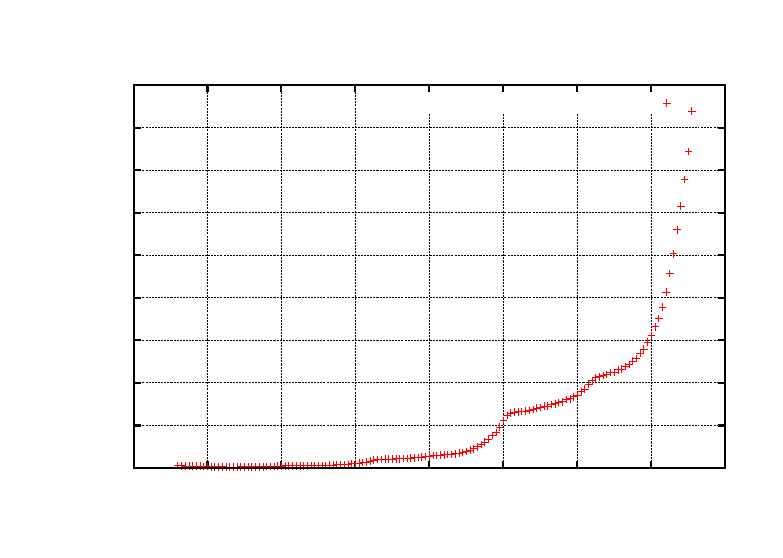
\includegraphics{abs}}%
    \gplfronttext
  \end{picture}%
\endgroup

	\caption{Absorptionsspektrum (380-700nm) von reinem Wasser. (1997). \url{http://omlc.org/spectra/water/abs/}}
	\label{fig:abs}
\end{figure}




\subsection{Nichtinvertierbarer Operationsverstärker}

Dabei handelt es sich von der Grundschaltung her um einen Operationsverstärker.
Diese finden sehr viel Anwendung in allen möglichen Bereichen, zum Beispiel der Mess-und Regelungstechnik. 
Allgemeine Eigenschaften dieser Bauteile sind, eine sehr große Verstärkung von Eingangsignalen, sowie ein hoher Eingangs und dazu vergleichsweise geringer Ausgangswiderstand.
Das allgemeine Verstärkersymbol ist ein Dreieck in es werden darin auch die beiden
Eingänge mit + und - gekennzeichnet.
Der - Eingang wird als invertierbarer Eingang und 
der + Eingang als nicht invertierbarer Eingang bezeichnet.
Das eigentliche Bauteil des Verstärkters ist sehr komplex und es lohnt sich nicht hier 
weiter darauf einzugehen.
Entscheident ist hier nur die Formel für den Verstärkungsfaktor $v$ für den verwendeten 
Nichtinvertierbaren Verstärkers. Für diese gilt:
\begin{align}
 v = 1 + \frac{R_2}{R_1}
\end{align}
Wichtig ist also nur die für den jeweiligen Bedarf richtige Wahl des Widerstandverhältnisses.
Eine weitere Eigenschaft des Nichtinvertierbarer Verstärker ist, dass die Phase des Eingangs
und Ausgangssignals gleich sind. Diese Eigenschaft ist für das Echolot wichtig.


\subsection{Schichtung eines Sees}

Man unterscheidet drei Tiefenschichten eines Sees.
Diese haben alle verschiedene physikalische, chemische, sowie biologische Eigenschaften. Die Grenzen zwischen diesen Schichten sind kontinuierlich und oftmals schwer zu unterscheiden, insbesondere bei flachen Seen.
Die oberste Schicht wird auch Epilimnion genannt. 
Im Sommer lagert sich dort warmes Wasser mit geringer Dichte ab.
Während dieser Zeit kommt es daher nur zu einem geringen Austausch des Wassers
mit tieferen Schichten, sodass in diesen immer weniger Sauerstoff zu finden ist.
Zudem findet effektiver Wärmeaustausch mit tieferen Schichten dann nur noch Aufgrund von vergleichsweise
kleinen Strömungen statt. Diese werden durch Wind oder im geringen Maße durch Sonneneinstrahlung erzeugt. 
Das Klima ist daher ein entscheidender Faktor für die Dicke dieser Schicht.
Diffusiver Wärmetransport hingegen ist ein sehr langsamer
Prozess, so vergeht zum Beispiel etwa ein Monat für das Bilden einer etwa 1 m dicken Schicht vergleichsweise wärmeren Wassers.
Ab einer Tiefe von circa 10 m führt dies insgesamt zur Entstehung eines größeren Temperaturgradienten im Sommer und 
zur Entstehung der mittleren Schicht (Thermonokline). Dabei handelt es sich um eine recht dünne  Übergangschicht. Diese trennt die obere Schicht von größeren Tiefen. 
\cite{schicht}
%http://www.wiley-vch.de/books/sample/3527321314_c01.pdf
\newline
Das Epilimnion  ist klarerweise die wärmste und besitzt den größten pH wert, da es hier zu Kontakt mit der Atmosphäre kommt. In Folge dessen lösen sich Gase wie Kohlenstoffdioxid, sodass beispielsweise Kohlensäure entsteht. Außerdem besitzt diese Schicht auch den größten Sauerstoffgehalt. Hier sind auch die meisten phototrophen Planktonarten zu finden, denn es ist der hellste Bereich des Sees. Abgestorbenes Plankton lagert sich dann auf den Grund des Sees ab und steht anderen Lebewesen als Nahrung zur Verfügung.
\newline
Die unterste Schicht wird auch Hypolimnion genannt.
Im Sommer ist dies die kälteste Schicht und auch die mit dem geringsten Sauerstoffgehalt. 
Ganz grundsätzlich unterliegen diese Schichten jahreszeitlichen Schwankung in ihrer Dicke.
Es kommt dann im Herbst zu einer teilweisen Durchmischung zwischen Hypolimnion und dem Epilimnion, da sich das Wasser an der Oberfläche abkühlt und absinkt.
Im Winter, wenn die Außentemperaturen längere Zeit unter Null Grad gewesen sind, ist das Hypolimnion die wärmste Schicht, da Wasser mit einer Temperatur von 4 Grad am dichtesten ist. 
Im Extremfall liegt dann eine vollständige Durchmischung aller Schichten vor.
Aus diesem Grund ist eine (Temperatur-) Schichtung bei permanent gefrohrenen Gewässern nicht vorzufinden.
\newline
In Grafik \ref{fig:schichtung} sind zur Veranschaulichung der Leitwert C, die Temperatur T und der Sauerstoffgehaltprofil des Arendsee (Sachsen Anhalt, Messung im September) dargestellt. 
Aufgrund der beinahe konstanten Temperatur im oberste sowie untersten Bereich kann man hier die drei oben geschilderten Schichten gut von einander trennen. Insbesondere erkennt man den starken Temperaturgradienten im Metalimnion, das hier zwischen 8 und 15 m liegt. 
Das Kabel, welches in unserem Experiment den Logger mit der Sonde verbindet hat eine länge von circa 8 m. Es ist also zu erwarten, dass wir beim Vermessenen des Sees grade an die Grenze des Epilimnions stoßen.


\begin{figure}[h]
	\centering
	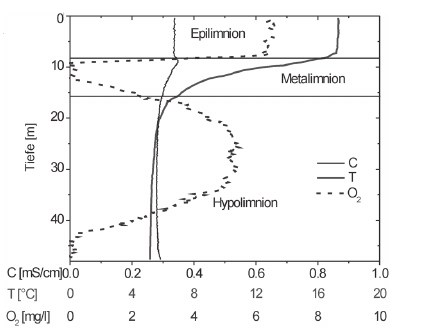
\includegraphics[height=10cm]{schicht.png}
	\caption{Leitwert $C$, Temperatur $T$ und Sauerstoff $O_2$ des Arendsees im September. Grafik entnommen aus \url{http://www.wiley-vch.de/books/sample/3527321314_c01.pdf}.}
	\label{fig:schichtung}
\end{figure}



\subsection{Ortsbestimmung}
\label{sec:theoort}
Um den Ort des Bootes zu bestimmen, verwendeten wir ein Geodimeter (s. Abb. \ref{fig:geodimeter}).
Dieses sendet einen Laserstrahl in eine bestimmte Richtung aus und misst, sobald er reflektiert wird die Flugdauer.
Daraus bestimmt es die Entfernung.
Die Richtung wird durch die Stellung des beweglichen Kopfes ermittelt.
Dafür wird beim Einschalten eine Referenzrichtung eingeschtellt, anhand derer die Abweichung bestimmt wird.
Das Gerät kann nun die relative Position zu dem eigenen Standort in verschiedenen Darstellungsweisen ausgeben: Zylinderkoordinaten und Kartesische Koordinaten.

Der Laser wird von einem Retroreflektor an einer Messstange reflektiert, welche mit an Bord genommen wird.
Ein Retroreflektor ist eine Anordnung von drei Spiegeln, welche jeweils im $90^\circ$-Winkel zueinander stehen.
Jeder einfallende Strahl wird so in die Herkunftsrichtung zurückgelenkt.\\
Als zweite Mögliche Ortsbestimmung wird das GPS System verwendet, dass durch Triangulation von Signalen einiger Sateliten die Position bestimmt.
Diese Methode ist vergleichsweise ungenau mit einer Genuigkeit von $\pm5\si{\meter}$, aber im Vergleich zur größe von Seen immernoch genau genug.
Die Implementierung dieser Methode wird im Kapitel \ref{sec:durchpos} weiter beschrieben.

Parallel zu dem direkten Speichern haben wir auch eine Smartphone-App erstellt, die ebenfalls die Position aufzeichet (s. Kapitel \ref{sec:app}).


\begin{figure}[h]
	\centering
	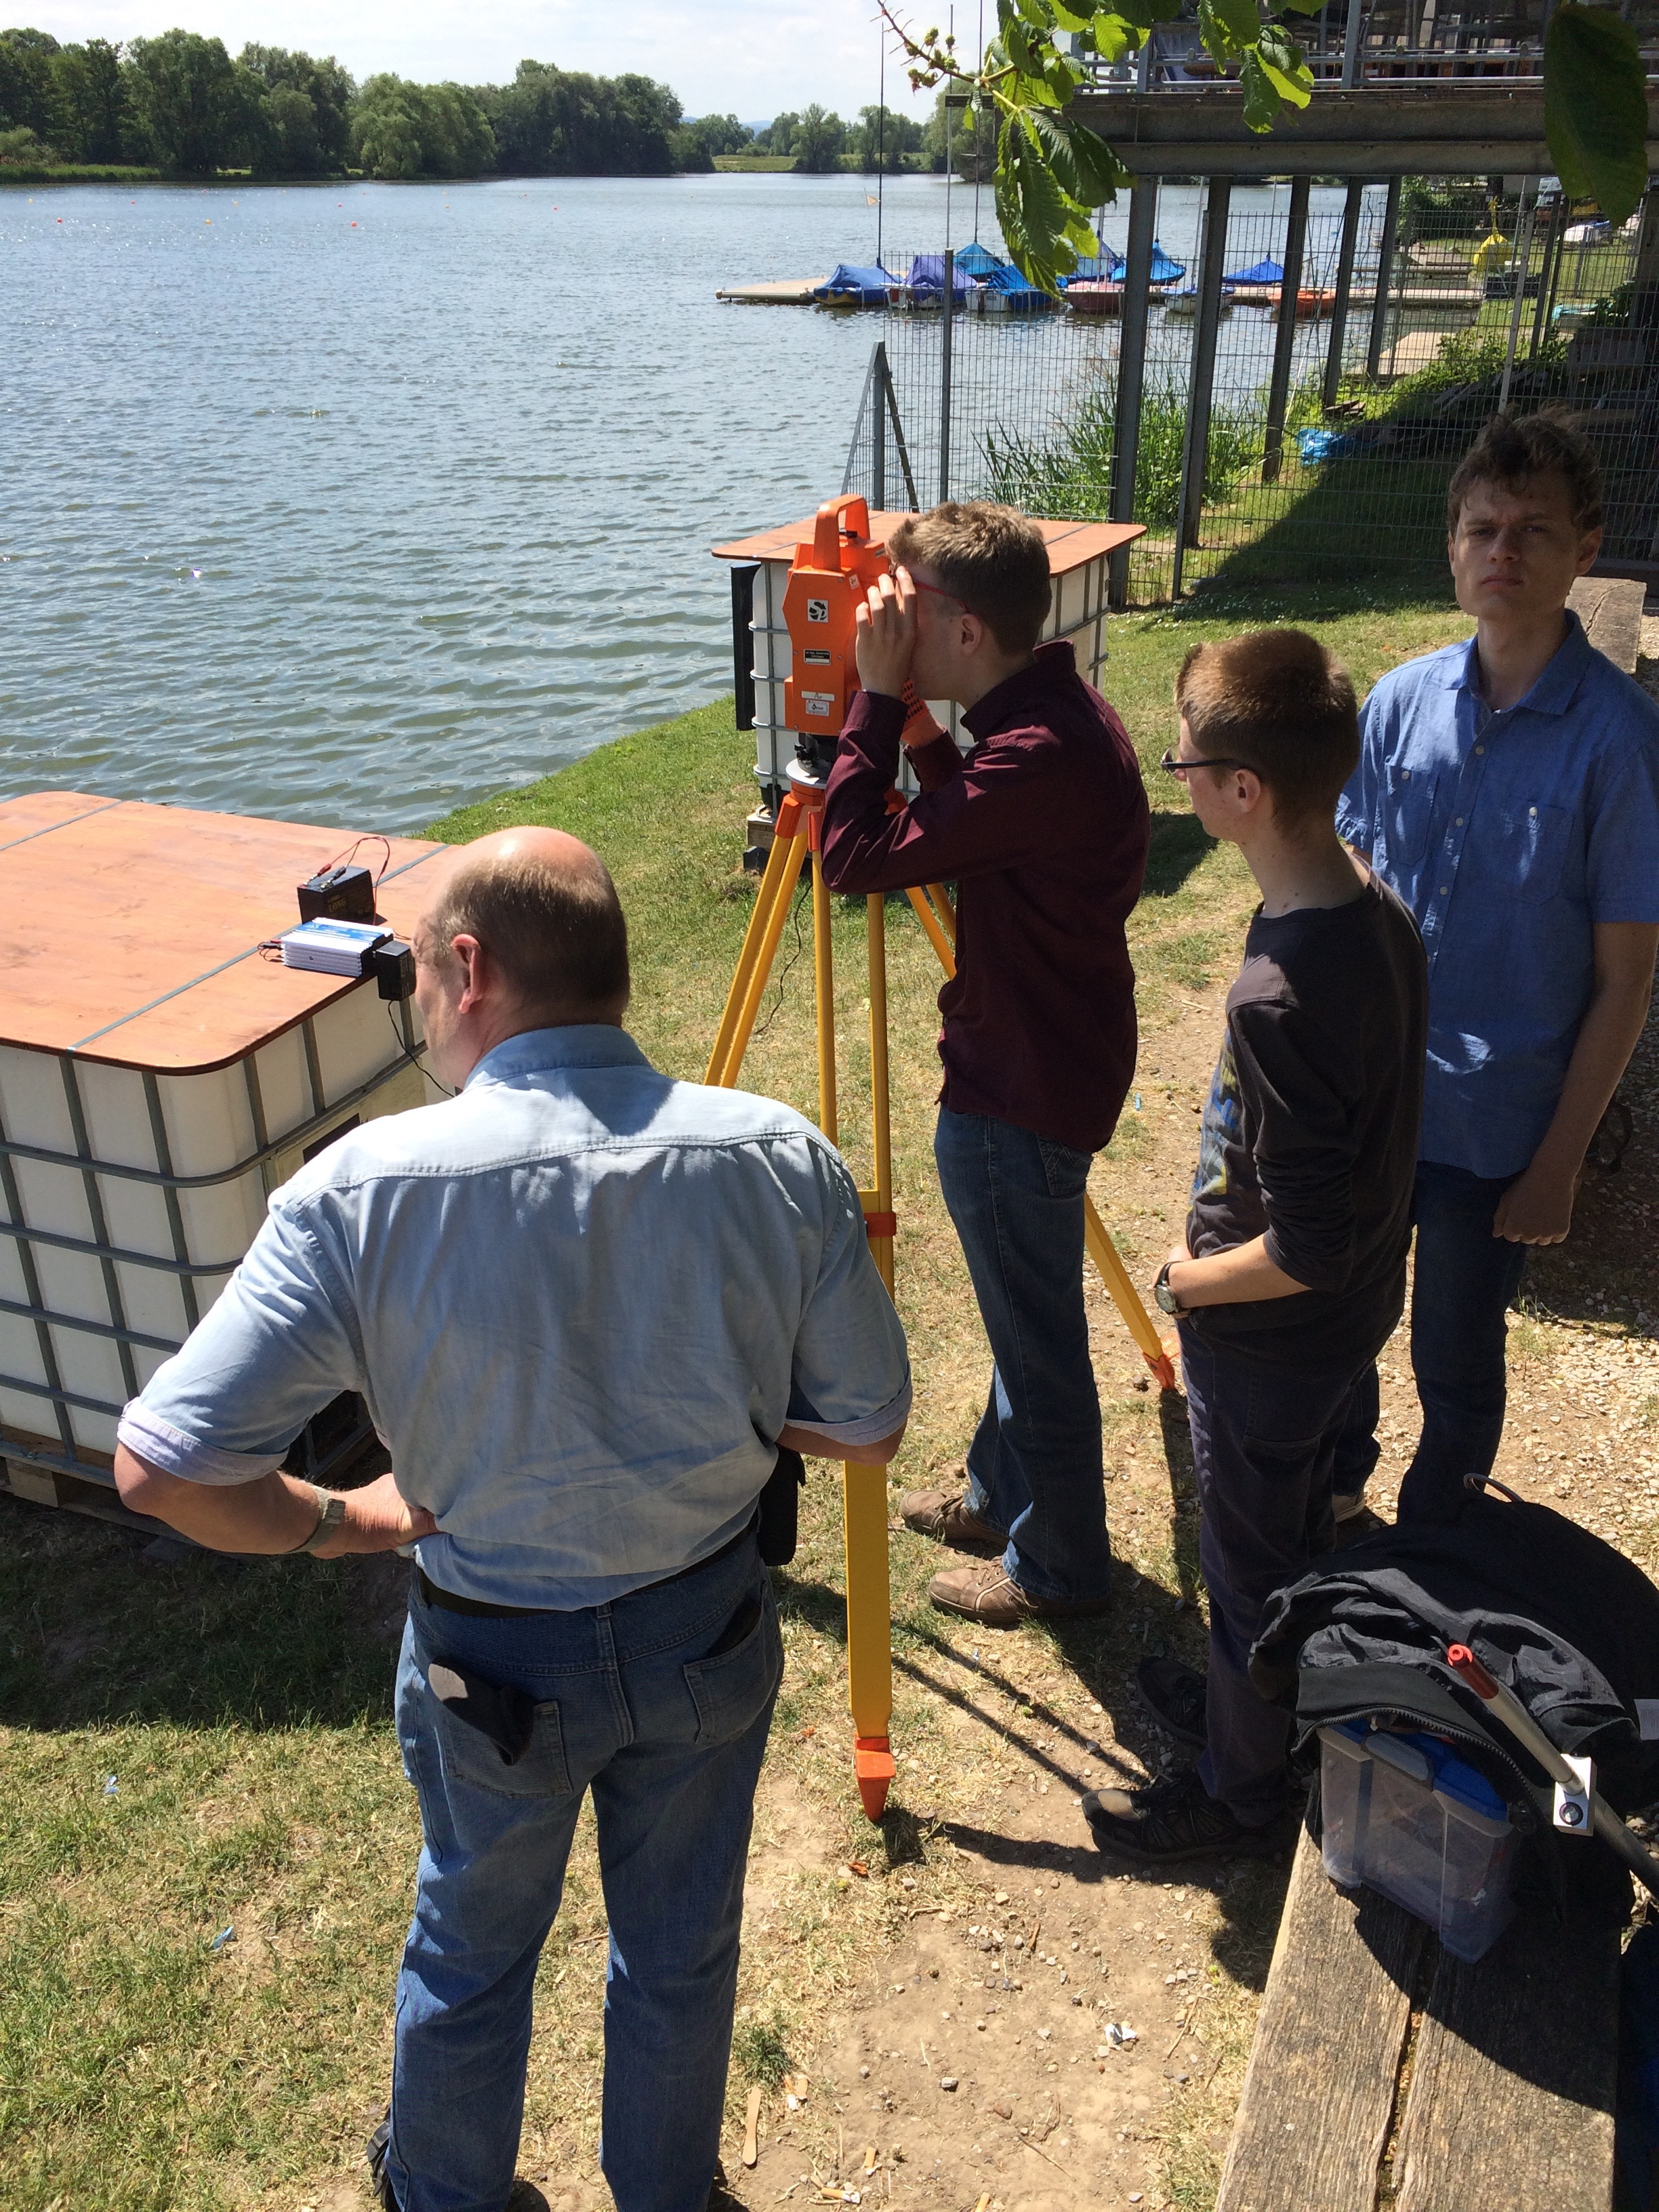
\includegraphics[height=10cm]{Fotos/Geodimeter}
	\caption{Kevin beim Einstellen des Geodimeters.}
	\label{fig:geodimeter}
\end{figure}


\subsection{Temperatur}
Die Temperatur wird mit einem Pt1000-Widerstand vermessen.
Der Name verrät, dass der Messfühler aus Platin ist und bei $0\si{\celsius}$ einen Widerstand von $R_0=1000\si{\ohm}$ hat.
Der Widerstand hängt so von der Temperatur $\vartheta>0\si{\celsius}$ ab
\begin{align}
	R(\vartheta)&=R_0\cdot\left(1 + A\vartheta + B\vartheta^2\right). \label{eq:Pt1000}
\end{align}
Diese Formel ist rein empirisch. 
Die zugehörigen Konstanten die in Eichmessungen ermittelt werden findet man in Tabelle \ref{tab:Pt1000}.

\begin{table}[!htb]
	\centering
	\begin{tabular}{|c|c|}
		\hline
		R$_0$ & $1000 ~ \si{\ohm}$\\
		A   & $3.9083 \cdot 10^{-3} ~ \si{\celsius^{-1}}$\\
		B   & $-5.775 \cdot 10^{-7} ~ \si{\celsius^{-2}}$\\
		\hline
	\end{tabular}
	\caption{Kennwerte des Widerstandsthermometers}
	\label{tab:Pt1000}
\end{table}

Durch Umstellen erhält man eine Fomel für die Temperatur in Grad Celsius
\begin{align}
 \vartheta = -\frac{A}{2 B} - \frac{1}{2 B \sqrt{R_0}} \sqrt{A^2 R_0  - 4 B R_0 + 4 B R    } .
\end{align}

Der Fehler der Temperaturmessung dieses Gerätes liegt bei
\begin{align}
	\Delta\vartheta=\pm (0.3~\si{\celsius}+0.005\vartheta)~.
	\label{eq:Pt1000_fehler}
\end{align}


\section{Durchführung}
\label{sec:durchfuehrung}

\subsection{Aufbau des Datenloggers}
Der Datenlogger ist speziell für diese Aufgabe entworfen und gebaut.
Die Basis für diesen ist das XMC4500 RelaxKit von der Firma Infoneon$^\copyright$ mit einem 32bit Mikrocontroller.
Dieser wurde mithilfe der Software Dave$^\copyright$ von der gleichen Firma programmiert.\\
Zur Bestimmung der am Controller anliegenden Spannung wird ein integrierter Analog Digital Converter (ADC) verwendet.
Dieser berechnet die Spannung über ein iteratives Verfahren, in dem er die anliegende Spannung mit einer Refferenzspannung vergleicht.
Die Refferenzspannung wird bei jedem Schritt halbiert oder um die Hälfte erhöht jeh nach dem, ob die zu messende Spannung kleiner oder größer ist.
Der ADC hat eine Auflösung von 12bit %ref auf Datenblatt
, somit hat das Verfahren auch 12 Schritte.
Die Refferenzspannung liegt bei 3.3\si{\volt}, welche vom Board intern bereitgestellt wird.
Diese Spannung ist auch die Maximalspannung, die an einen Pin des Mikrocontrollers angelegt werden darf, ohne ihn zu zerstören.
Aus diesem Verfahren ergibt sich bei 12bit einen minimal von Null verschiedene Spannung von $B=\frac{3.3\si{\volt}}{2^{12}}=8.06\times10^{-4}\si{\volt}$, welche als Bereichsbreite $B$ bezeichnet wird.
Somit kann die Spannung aus dem ausgegebenen ADCWert über die Bereichsbreite berechnet werden
\begin{align}
	U=\text{ADCWert}\cdot B.\label{eq:ADCwert}
\end{align}
Für die Sensoren werden verschiedene Schaltungen verwendet, die im Folgenden näher erläutert.
Bei allen Schaltungen ist zu beachten, dass in allen Fällen die Massen gekoppelt sind.\\
Die Daten werden in Form einer ASCII Datei auf einer SD-Karte gespeichert, um sie am Computer später leichter in einem Plotprogramm bearbeiten kann.
Dies sorgt aber für ein größeres Datenvolumen.
Jede Datei trägt, zur besseren Identifikation, den aktuellen Monat, Tag, Stunde und Minute als Namen (MMDDHHMM.dat).
In der Datei wird die Zeit in Millisekunden, die ADCWerte von Temperatur, Photodiode und Druck, sowie die Berechneten Werte der Temperatur, Intensität, Druck und Tiefe berechnet aus dem aktuellen Luftdruck eingetragen.


\subsubsection{Temperaturmessung}
\begin{figure}[!h]
\centering
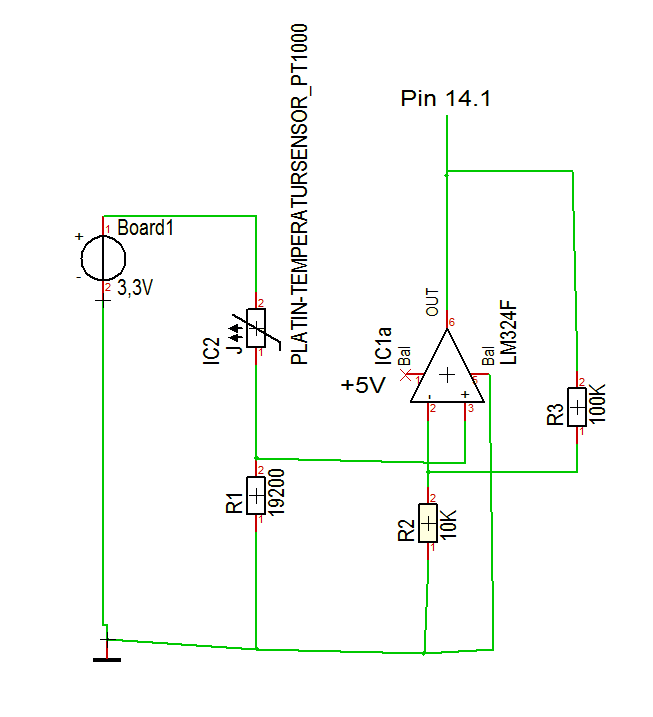
\includegraphics[width=0.5\textwidth]{Fotos/PT1000Schaltung.png}
\caption{Beschaltung des PT1000 Temperaturwiderstandes mit Vorwiderstand und Verstärkerschltung.}
\label{fig:PT1000Schaltung}
\end{figure}
Für die Messung der Temperatur wird mit einem PT1000 Temperaturwiderstand gearbeitet.
Dieser benötigt eine spezielle Beschaltung, da durch ihn nur ein geringer Strom fließen darf.
Aus diesem Grund muss die am PT1000 abfallende Spannung noch verstärkt werden.
Dies geschieht mithilfe eines nichtinvertierenden Verstärkers. %ref aufquelle
Mit der Formel %ref auf Formel
ergibt sich bei der in der Abbildung \ref{fig:PT1000Schaltung} gezeigte Beschaltung eine Verstärkungsfaktor von 11.
Dieser Wert verstärkt somit die etwa 200\si{\milli\volt} auf 2\si{\volt}, was etwa in der Mitte des Messbereiches des ADC liegt.\\
Aus dem in der Abbildung \ref{fig:PT1000Schaltung} zu sehendem Widerstandsnetzwerk leitet sich die Formel
\begin{align}
	R_\text{PT1000}=\frac{R_1*U_\text{ADC}}{3.3\si{\volt}-U_\text{ADC}}
\end{align}
ab, wobei $U_\text{ADC}$ die Spannung ist, welche mit der Formel \eqref{eq:ADCwert} aus dem ADCWert berechnet wird.
Zur anschließenden Berechnung der Temperatur aus den gemessenen Widerständen wird die Formel %ref auf Formel
verwendet.\\
Der Sensor ist zwecks Wasserdichtigkeit mit einem dünnen Film Klebstoff beschichtet.
Dieser sollte nur die Reaktionszeit beeinflussen.

\subsubsection{Lichtmessung}
\begin{figure}[!h]
\centering
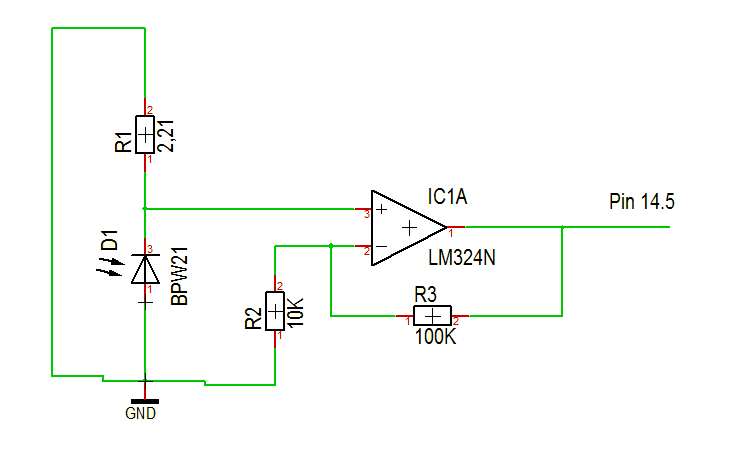
\includegraphics[width=0.5\textwidth]{Fotos/PhotodiodeSchaltung.png}
\caption{Beschaltung der Photodiode mit Widerstand und Verstärkerachaltung.}
\label{fig:PhotodiodeSchaltung}
\end{figure}
\begin{figure}[!h]
\centering
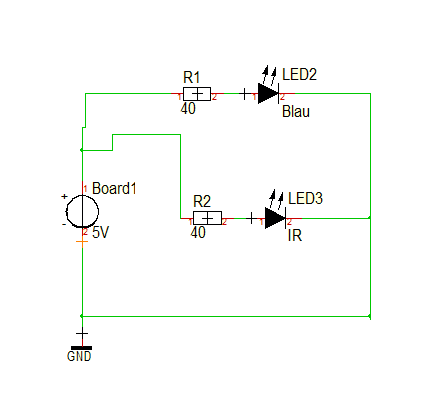
\includegraphics[width=0.6\textwidth]{Fotos/LEDSchaltung.png}
\caption{Beschaltung der LEDs für die Messung der Absorbtion.}
\label{fig:LEDSchaltung}
\end{figure}
Für die Lichtmessung wird eine Photodiode als Intensitätsabhängige Stromquelle verwendet.
Die Schaltung ist in der Abbildung \ref{fig:PhotodiodeSchaltung} zu sehen.
Der Stromkreis besteht aus der Photodiode als Stromquelle und einem Widerstand, um den Strom in eine Messbare Spannung zu wandeln.
Da in den See nicht viel Licht eintritt wird die sich ergebene Spannung noch über einen nichtinvertierenden Verstärker nach der Gleichung %ref auf Gleichung
mit einem Faktor 11 Verstärkt.
Die Spannung wird dann wieder mit der Gleichung \eqref{eq:ADCwert} berechnet.\\
Um die Absorbtion in verschiedenen Spektren zu Messen hat die Messonde eine Blaue und eine Infrarote LED %ref auf die Datenblätter
mit mittleren Wellenlängen von $\lambda_\text{Blau}=\si{\nano\meter}$ und $\lambda_\text{IR}=\si{\nano\meter}$. %ref auf Datenblatt
Die LEDs werden ebenfalls von der boardinternen Spannungsquelle versorgt und wie in der Abbildung \ref{fig:LEDSchaltung} zu sehen mit entsprechenden Vorwiderständen beschaltet.\\
Im Programm werden die Linien von den jeweiligen LEDs und den Phasen ohne LEDbetrieb getrennt gespeichert.

\subsubsection{Druckmessung}
Der Druck wird durch einen Absolutdrucksensor in einer Messbrücke bestimmt.
Die Schaltung wurde von der Geophysik bereitgestellt und dierekt an dem Pin 14.2 am Board angeschlossen.
Zu dem muss die Masse von der externen Schaltung mit der Masse des Boards gekoppelt werden.
Die Messbrücke ist mit einem Potentiometer bei einer Spannung von 1\si{\volt} auf einen Druck von 1001HPa geeicht.
Bei der Messbrücke haldelt es sich um  eine Wiedstonbrücke, die bereits vom Werk aus geeicht ist.
Die ausgebene Spannung ist somit proportional zum angewanten Druck.
Der Luftdruck liegt bei etwa 1024HPa und in einer Tiefe von 10\si{\meter} hat sich der Druck um 1000HPa erhöht, und damit auch die Spannung um 1\si{\volt}.
Somit liegt der Spannungsbereicht in dem akzeptablen Bereich des ADC.

\subsubsection{Echolotmessung}
Mithilfe von zwei Piezokristallen wird eine Echolotmessung realisiert.
Die Kristalle haben eine Resonanzfrequenz von 40\si{\kilo\hertz} und liegen somit im Ultraschallbereich.
Das Senderkristall wird mithilfe von PWM (Puls Width Modulation) mit einem Signal von maximal +3.3\si{\volt} versorgt, um diese Maxiamlspannung zu erhöhen wird das Kristall über ein MosFettransistor an +24\si{\volt} betrieben.%Schaltung hinzufeugen
Um die Tiefe zu Messen, muss ein klar definiertes Signal ausgesendet werden, hierzu werden 20 Schwingungen auf das Senderkristall gegeben.\\
Das Empfängerkristall wird über einen Verstärker dierekt an den ADC angeschlossen.
Für die Messung der Tiefe wird die Laufzeit der Wellen vom Aussenden bis zum Empfangen gemessen und daraus die Entfernung berechnet.
Zur Bestimmung der Bodenbeschaffenheit wird zudem das ganze ausgesendete Signal aufgezeichnet und anschließend analysiert.

\subsection{Positionsbestimmung via GPS und Geodimeter}
\label{sec:durchpos}
Die Bestimmung der Position wird zum einen mithilfe eines Geodimeters durchgeführt.
Dieses berechnet, wie im Kapitel\ref{sec:theoort} beschrieben, die Position durch eine genaue Berechnung der Entfernung und des Winkels mithilfe eines Lasers und einem Retroreflektor.\\
Diese Messmethode ist sehr genau, benötigt aber zwei Teams, eines das an Land das Geodimeter bedient, sowie die Koordinaten notiert und eines, dass auf dem Boot den Retroreflektor positioniert.
Als alternative hierzu wird ein GPS in den Datenlogger implementiert, welches bei jeder Messung die aktuellen globalen Koordinaten in die Messdatei schreibt.
Hierzu wird ein GPS von Garmin$^{\copyright}$ verwendet, welches in der Geophysik vorhanden war genutzt.
Dieses besitzt eine RS232 Schnittstelle, welche mithilfe eines selbstgebauten Pegelkonverters die $\pm6\si{\volt}$ auf TTL Signale mit einem maximalen Pegel von 3.3\si{\volt} und einem minimalen Pegel von 0\si{\volt} konvertiert.
Dies geschieht über 5 Dioden und einem Pulldownwiderstand, um eine kleine Last zu erzeugen, die das Signal nicht verzerrt.
Anschließend werden die Daten vom Mikrocontroller über eine UART Schnittstelle bei einer Baudrate von 9600$~$Baud eingelesen.
Das GPS sendet die aktuellen Koordinaten mit der aktuellen Atomzeit als ASCII Text jede Sekunde an den Logger.
Mithilfe der Zeit kann die RTC (Realtimeclock) einmalig auf Atomuhrzeit eingestellt werden.

\subsection{Messdurchführung}

Zur Vermessung eines Sees ist es notwendig, zunächst den Bereich, den man vermessen möchte sinnvoll einzuschränken und sich eine Rasterung zu überlegen.
Dabei ist zu bedenken, dass für jeden Messpunkt ca. 3-5min eingerechnet werden müssen.
Auch müssen die Positionen, sofern sie mit dem Geodimeter ermittelt werden sollen, alle von einem Punkt am Ufer aus sichtbar sein.
Man könnte zwar das Geodimeter umstellen, jedoch würde dies zu einer enorm vergrößerten Unsicherheit des Ortes führe.

Die eigentliche Messung besteht darin, dass der Ruderer an einer Stelle anhält und den Messstab für das Geodimeter hochhält und ausrichtet.
Wird die Einzelmessung der App gleichzeitig mit dem Datenlogger gestartet, so wird zu den GPS-Daten der App gleich der Dateiname der Messreihe gespeichert.
Ist nun die Messung gestartet, so wird die Sonde langsam ins Wasser gelassen.
Um eine signifikante Menge an Datenpunkten für alle Tiefen zu bekommen, darf man die Sonde mit einer Sinkgeschwindigkeit von höchstens 10cm/s herunterlassen.
Erreicht die Sonde den Boden, so muss die Messung beendet werden, da sich sonst gegebenenfalls Schlamm um die Sensoren legt.
Kommt das Gewicht nicht auf dem Boden an, so kann die Sonde wieder nach oben gezogen werden um die doppelte Anzahl an Messwerten für die jeweilige Tiefe zu bekommen.

Erreicht die Sonde in diesem Fall wieder die Oberfläche, so wird die Messung beendet.
Dies ist notwendig, da der Lichtsensor an der Oberfläche durch die Sonneneinstrahlung eine zu hohe Spannung liefert und so den ADC übersteuert.

\subsection{Smartohone-App}
\label{sec:app}
Da bei der ersten Messung schon das Abfahren des relativ kleinen Göttinger Kiessees in einem regelmäßigen Raster nicht leicht war, haben wir eine App für das Smartphone erstellt.
Das GPS-Modul des Smartphones liefert die aktuelle Position und stellt sie auf einer Karte dar.
Nun gibt es zwei Möglichkeiten:
\begin{itemize}
	\item Multi-Messung: Die Position wird ständig getrackt.
		Sobald sie sich verändert, wird diese in eine Datei geschrieben.
	\item Einzelmessung: Dies kann parallel zu der Multi-Messung passieren.
		Hierbei wird nur auf Knopfdruck auf den Button "`Einzelmessung"' ein einzelner Ort in eine andere Datei geschrieben.
		Außerdem wird die Position auf der Karte mit einer Stecknadel markiert und um die Position wird ein Radius eigezeichnet, der sich über einen Schieberegler einstellen lässt.
		Dies hat den Vorteil, dass man variabel die Rasterung anpassen kann.
\end{itemize}

Die App zeigt (wie in Abb. \ref{fig:appDetail} zu sehen) auch die Anzahl der aufgenommenen Datenpunkte an und die beiden Dateien, welche bei den Messungen angelegt werden.

Wurde die Messung an einem Ort nun beendet, kann man einfach so lange in eine Richtung fahren, bis man den roten Kreis um den letzten Datenpunkt erreicht hat.
Im Verlauf der Messung wird nun der ganze See systematisch mit den Kreisen überdeckt.

Am Ende des Messtages kann mit dem Knopf "`Senden"' nun eine Tabelle (s. Abb. \ref{fig:appTabelle}) geöffnet werden, welche die vorhandenen Dateien anzeigt.
Tippt man nun auf eine der Zeilen, so wird eine Mail erstellt, die schon voreingestellt die Mailadressen, Betreff und Inhalt, sowie die angehängte Datei besitzt.
Diese kann nun bequem mit einem Tippen versandt werden.


\begin{figure}[h]
  \centering
  \subfigure[Einzelne Datenpunkte an einer Stelle des Sees.\label{fig:appDetail}]
  {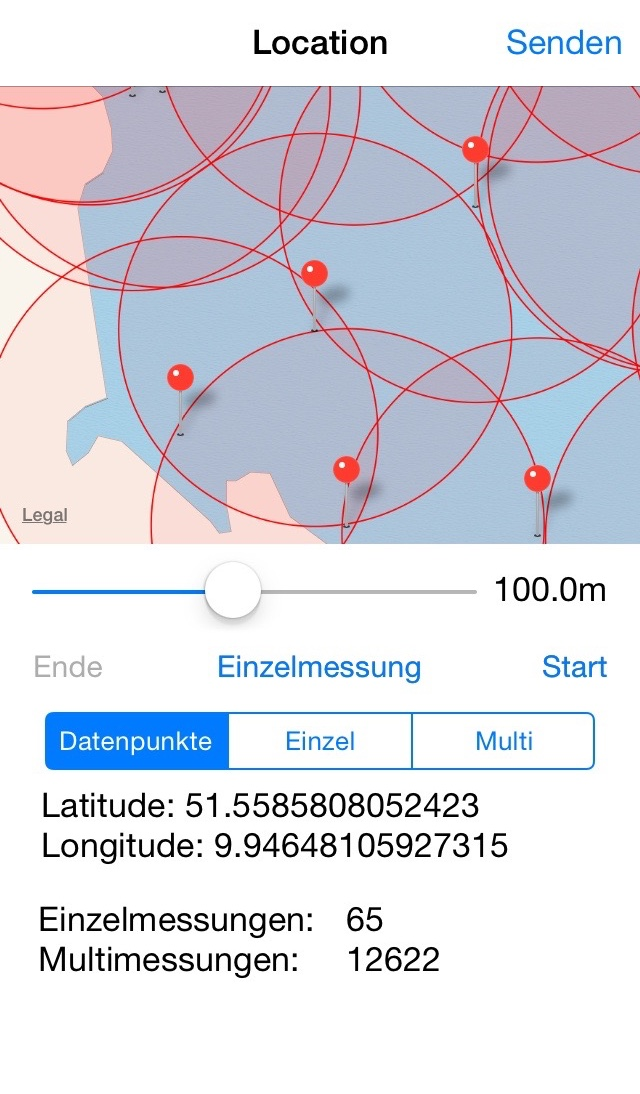
\includegraphics[width=0.32\textwidth]{Fotos/AppSeeDetail}}
  \hfill
  \subfigure[Übersicht über alle aufgenommenen Messpunkte in der App.\label{fig:appGesamt}]
  {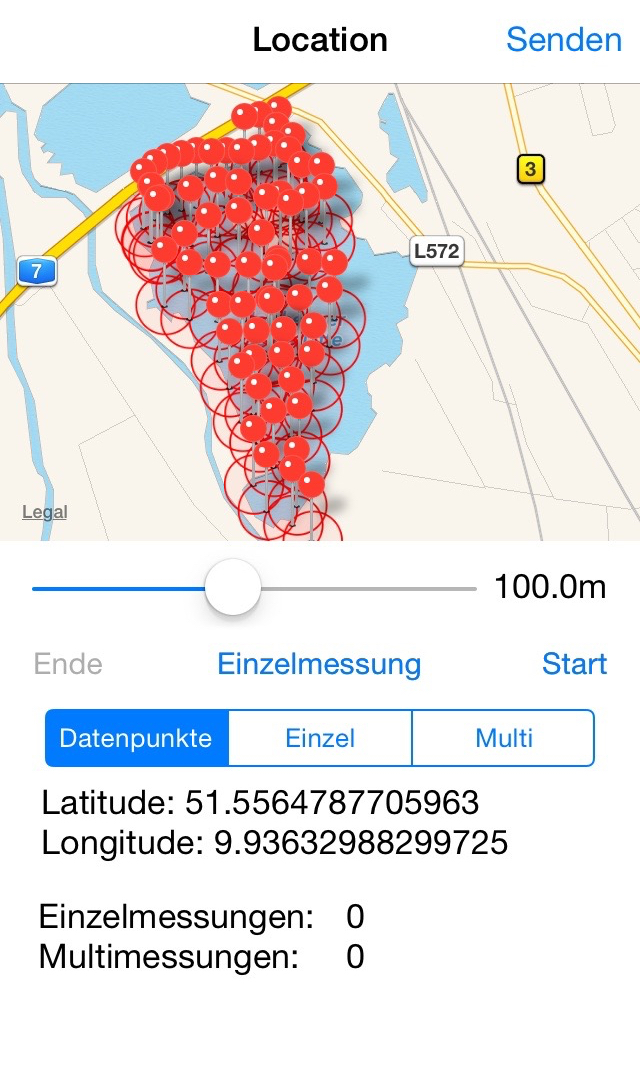
\includegraphics[width=0.32\textwidth]{Fotos/AppSeeKomplett}}
  \hfill
  \subfigure[Auswahl der zu versendenden Datei.\label{fig:appTabelle}]
  {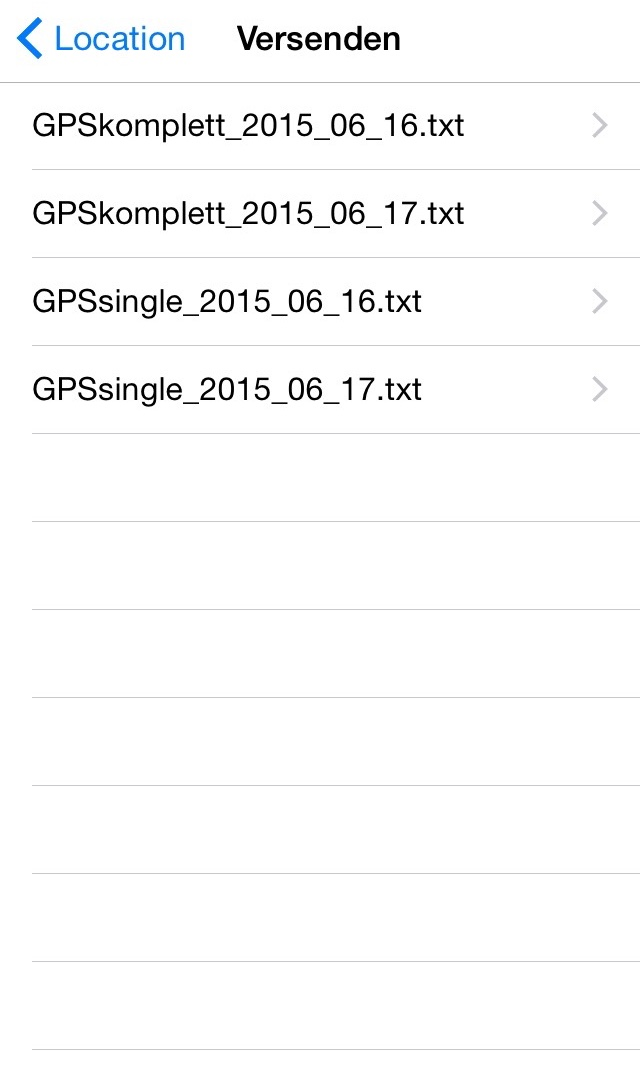
\includegraphics[width=0.32\textwidth]{Fotos/AppVersenden}}
  \caption{Screenshots der App.}
  \label{fig:appScreenshots}
\end{figure}


\section{Auswertung}
\label{sec:auswertung}

\subsection{Ortsbestimmung}

Unsere Befürchtung, dass das GPS-Signal zu ungenau ist, stellte sich als ungenau heraus.
Wir nutzten bei der zweiten Messung gleichzeitig einen GPS-Logger und die selbstgeschriebene Handy-App.
Durch Vergleich der beiden Messdaten erkennt man, dass sie sehr gut miteinander übereinstimmen.
Dies ist vielleicht auch zu erwarten, da beide ähnliche Signale bekamen.

Der GPS-Logger zeigte die Genauigkeit auf dem Display an, welche fast immer 3m betrug.
Diese hohe Genauigkeit, welche sich unter "`Normalbedingungen"' nur selten erreichen lässt, wird dadurch erklärt, dass wir auf einer weiten Fläche ohne große Hindernisse waren.
Somit gab es nichts, was die Signale der Satelliten reflektieren oder blockieren konnte.


In Abb. \ref{fig:einzelGPSGoe} sind alle Messpunkte am Göttinger Kiessee aufgetragen.
Diese wurden mit dem Geodimeter bestimmt.
Als Vergleich sind die Daten, die wir mit einer anderen App aus dem App-Store\textsuperscript{\textregistered}  aufgenommen haben in Abb. \ref{fig:GPSGoe} aufgetragen.
Diese wurden Durchgehend aufgezeichnet, jedoch kann man an den Umkehrpunkten erkennen, dass die Positionen ungefähr übereinstimmen.

\begin{figure}[h]
\centering
% GNUPLOT: LaTeX picture with Postscript
\begingroup
  \makeatletter
  \providecommand\color[2][]{%
    \GenericError{(gnuplot) \space\space\space\@spaces}{%
      Package color not loaded in conjunction with
      terminal option `colourtext'%
    }{See the gnuplot documentation for explanation.%
    }{Either use 'blacktext' in gnuplot or load the package
      color.sty in LaTeX.}%
    \renewcommand\color[2][]{}%
  }%
  \providecommand\includegraphics[2][]{%
    \GenericError{(gnuplot) \space\space\space\@spaces}{%
      Package graphicx or graphics not loaded%
    }{See the gnuplot documentation for explanation.%
    }{The gnuplot epslatex terminal needs graphicx.sty or graphics.sty.}%
    \renewcommand\includegraphics[2][]{}%
  }%
  \providecommand\rotatebox[2]{#2}%
  \@ifundefined{ifGPcolor}{%
    \newif\ifGPcolor
    \GPcolortrue
  }{}%
  \@ifundefined{ifGPblacktext}{%
    \newif\ifGPblacktext
    \GPblacktexttrue
  }{}%
  % define a \g@addto@macro without @ in the name:
  \let\gplgaddtomacro\g@addto@macro
  % define empty templates for all commands taking text:
  \gdef\gplbacktext{}%
  \gdef\gplfronttext{}%
  \makeatother
  \ifGPblacktext
    % no textcolor at all
    \def\colorrgb#1{}%
    \def\colorgray#1{}%
  \else
    % gray or color?
    \ifGPcolor
      \def\colorrgb#1{\color[rgb]{#1}}%
      \def\colorgray#1{\color[gray]{#1}}%
      \expandafter\def\csname LTw\endcsname{\color{white}}%
      \expandafter\def\csname LTb\endcsname{\color{black}}%
      \expandafter\def\csname LTa\endcsname{\color{black}}%
      \expandafter\def\csname LT0\endcsname{\color[rgb]{1,0,0}}%
      \expandafter\def\csname LT1\endcsname{\color[rgb]{0,1,0}}%
      \expandafter\def\csname LT2\endcsname{\color[rgb]{0,0,1}}%
      \expandafter\def\csname LT3\endcsname{\color[rgb]{1,0,1}}%
      \expandafter\def\csname LT4\endcsname{\color[rgb]{0,1,1}}%
      \expandafter\def\csname LT5\endcsname{\color[rgb]{1,1,0}}%
      \expandafter\def\csname LT6\endcsname{\color[rgb]{0,0,0}}%
      \expandafter\def\csname LT7\endcsname{\color[rgb]{1,0.3,0}}%
      \expandafter\def\csname LT8\endcsname{\color[rgb]{0.5,0.5,0.5}}%
    \else
      % gray
      \def\colorrgb#1{\color{black}}%
      \def\colorgray#1{\color[gray]{#1}}%
      \expandafter\def\csname LTw\endcsname{\color{white}}%
      \expandafter\def\csname LTb\endcsname{\color{black}}%
      \expandafter\def\csname LTa\endcsname{\color{black}}%
      \expandafter\def\csname LT0\endcsname{\color{black}}%
      \expandafter\def\csname LT1\endcsname{\color{black}}%
      \expandafter\def\csname LT2\endcsname{\color{black}}%
      \expandafter\def\csname LT3\endcsname{\color{black}}%
      \expandafter\def\csname LT4\endcsname{\color{black}}%
      \expandafter\def\csname LT5\endcsname{\color{black}}%
      \expandafter\def\csname LT6\endcsname{\color{black}}%
      \expandafter\def\csname LT7\endcsname{\color{black}}%
      \expandafter\def\csname LT8\endcsname{\color{black}}%
    \fi
  \fi
  \setlength{\unitlength}{0.0500bp}%
  \begin{picture}(7200.00,5040.00)%
    \gplgaddtomacro\gplbacktext{%
      \csname LTb\endcsname%
      \put(2791,704){\makebox(0,0)[r]{\strut{}-700}}%
      \put(2791,1213){\makebox(0,0)[r]{\strut{}-600}}%
      \put(2791,1722){\makebox(0,0)[r]{\strut{}-500}}%
      \put(2791,2231){\makebox(0,0)[r]{\strut{}-400}}%
      \put(2791,2740){\makebox(0,0)[r]{\strut{}-300}}%
      \put(2791,3248){\makebox(0,0)[r]{\strut{}-200}}%
      \put(2791,3757){\makebox(0,0)[r]{\strut{}-100}}%
      \put(2791,4266){\makebox(0,0)[r]{\strut{} 0}}%
      \put(2791,4775){\makebox(0,0)[r]{\strut{} 100}}%
      \put(2923,484){\makebox(0,0){\strut{}-100}}%
      \put(3177,484){\makebox(0,0){\strut{}-50}}%
      \put(3432,484){\makebox(0,0){\strut{} 0}}%
      \put(3686,484){\makebox(0,0){\strut{} 50}}%
      \put(3941,484){\makebox(0,0){\strut{} 100}}%
      \put(4195,484){\makebox(0,0){\strut{} 150}}%
      \put(4449,484){\makebox(0,0){\strut{} 200}}%
      \put(4704,484){\makebox(0,0){\strut{} 250}}%
      \put(4958,484){\makebox(0,0){\strut{} 300}}%
      \put(2021,2739){\rotatebox{-270}{\makebox(0,0){\strut{}y [m]}}}%
      \put(3940,154){\makebox(0,0){\strut{}x [m]}}%
    }%
    \gplgaddtomacro\gplfronttext{%
      \csname LTb\endcsname%
      \put(3971,877){\makebox(0,0)[r]{\strut{}Messpunkte}}%
    }%
    \gplbacktext
    \put(0,0){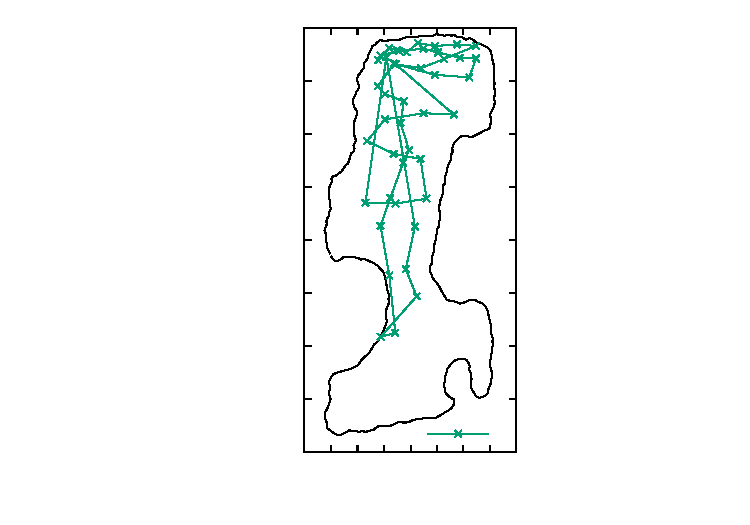
\includegraphics{karteGoe}}%
    \gplfronttext
  \end{picture}%
\endgroup

\caption{Positionen der Messungen am 10.6.2015 auf dem Göttinger Kiessee gemessen mit dem Geodimeter.}
\label{fig:einzelGPSGoe}
\end{figure}
\begin{figure}[h]
\centering
% GNUPLOT: LaTeX picture with Postscript
\begingroup
  \makeatletter
  \providecommand\color[2][]{%
    \GenericError{(gnuplot) \space\space\space\@spaces}{%
      Package color not loaded in conjunction with
      terminal option `colourtext'%
    }{See the gnuplot documentation for explanation.%
    }{Either use 'blacktext' in gnuplot or load the package
      color.sty in LaTeX.}%
    \renewcommand\color[2][]{}%
  }%
  \providecommand\includegraphics[2][]{%
    \GenericError{(gnuplot) \space\space\space\@spaces}{%
      Package graphicx or graphics not loaded%
    }{See the gnuplot documentation for explanation.%
    }{The gnuplot epslatex terminal needs graphicx.sty or graphics.sty.}%
    \renewcommand\includegraphics[2][]{}%
  }%
  \providecommand\rotatebox[2]{#2}%
  \@ifundefined{ifGPcolor}{%
    \newif\ifGPcolor
    \GPcolortrue
  }{}%
  \@ifundefined{ifGPblacktext}{%
    \newif\ifGPblacktext
    \GPblacktexttrue
  }{}%
  % define a \g@addto@macro without @ in the name:
  \let\gplgaddtomacro\g@addto@macro
  % define empty templates for all commands taking text:
  \gdef\gplbacktext{}%
  \gdef\gplfronttext{}%
  \makeatother
  \ifGPblacktext
    % no textcolor at all
    \def\colorrgb#1{}%
    \def\colorgray#1{}%
  \else
    % gray or color?
    \ifGPcolor
      \def\colorrgb#1{\color[rgb]{#1}}%
      \def\colorgray#1{\color[gray]{#1}}%
      \expandafter\def\csname LTw\endcsname{\color{white}}%
      \expandafter\def\csname LTb\endcsname{\color{black}}%
      \expandafter\def\csname LTa\endcsname{\color{black}}%
      \expandafter\def\csname LT0\endcsname{\color[rgb]{1,0,0}}%
      \expandafter\def\csname LT1\endcsname{\color[rgb]{0,1,0}}%
      \expandafter\def\csname LT2\endcsname{\color[rgb]{0,0,1}}%
      \expandafter\def\csname LT3\endcsname{\color[rgb]{1,0,1}}%
      \expandafter\def\csname LT4\endcsname{\color[rgb]{0,1,1}}%
      \expandafter\def\csname LT5\endcsname{\color[rgb]{1,1,0}}%
      \expandafter\def\csname LT6\endcsname{\color[rgb]{0,0,0}}%
      \expandafter\def\csname LT7\endcsname{\color[rgb]{1,0.3,0}}%
      \expandafter\def\csname LT8\endcsname{\color[rgb]{0.5,0.5,0.5}}%
    \else
      % gray
      \def\colorrgb#1{\color{black}}%
      \def\colorgray#1{\color[gray]{#1}}%
      \expandafter\def\csname LTw\endcsname{\color{white}}%
      \expandafter\def\csname LTb\endcsname{\color{black}}%
      \expandafter\def\csname LTa\endcsname{\color{black}}%
      \expandafter\def\csname LT0\endcsname{\color{black}}%
      \expandafter\def\csname LT1\endcsname{\color{black}}%
      \expandafter\def\csname LT2\endcsname{\color{black}}%
      \expandafter\def\csname LT3\endcsname{\color{black}}%
      \expandafter\def\csname LT4\endcsname{\color{black}}%
      \expandafter\def\csname LT5\endcsname{\color{black}}%
      \expandafter\def\csname LT6\endcsname{\color{black}}%
      \expandafter\def\csname LT7\endcsname{\color{black}}%
      \expandafter\def\csname LT8\endcsname{\color{black}}%
    \fi
  \fi
  \setlength{\unitlength}{0.0500bp}%
  \begin{picture}(7200.00,5040.00)%
    \gplgaddtomacro\gplbacktext{%
      \csname LTb\endcsname%
      \put(2037,704){\makebox(0,0)[r]{\strut{} 0}}%
      \put(2037,1111){\makebox(0,0)[r]{\strut{} 5e+06}}%
      \put(2037,1518){\makebox(0,0)[r]{\strut{} 1e+07}}%
      \put(2037,1925){\makebox(0,0)[r]{\strut{} 1.5e+07}}%
      \put(2037,2332){\makebox(0,0)[r]{\strut{} 2e+07}}%
      \put(2037,2740){\makebox(0,0)[r]{\strut{} 2.5e+07}}%
      \put(2037,3147){\makebox(0,0)[r]{\strut{} 3e+07}}%
      \put(2037,3554){\makebox(0,0)[r]{\strut{} 3.5e+07}}%
      \put(2037,3961){\makebox(0,0)[r]{\strut{} 4e+07}}%
      \put(2037,4368){\makebox(0,0)[r]{\strut{} 4.5e+07}}%
      \put(2037,4775){\makebox(0,0)[r]{\strut{} 5e+07}}%
      \put(2169,484){\makebox(0,0){\strut{}-2.5e+07}}%
      \put(2576,484){\makebox(0,0){\strut{}-2e+07}}%
      \put(2983,484){\makebox(0,0){\strut{}-1.5e+07}}%
      \put(3390,484){\makebox(0,0){\strut{}-1e+07}}%
      \put(3797,484){\makebox(0,0){\strut{}-5e+06}}%
      \put(4205,484){\makebox(0,0){\strut{} 0}}%
      \put(4612,484){\makebox(0,0){\strut{} 5e+06}}%
      \put(5019,484){\makebox(0,0){\strut{} 1e+07}}%
      \put(5426,484){\makebox(0,0){\strut{} 1.5e+07}}%
      \put(5833,484){\makebox(0,0){\strut{} 2e+07}}%
      \put(6240,484){\makebox(0,0){\strut{} 2.5e+07}}%
      \put(739,2739){\rotatebox{-270}{\makebox(0,0){\strut{}y [m]}}}%
      \put(4204,154){\makebox(0,0){\strut{}x [m]}}%
    }%
    \gplgaddtomacro\gplfronttext{%
      \csname LTb\endcsname%
      \put(5253,1097){\makebox(0,0)[r]{\strut{}GPS}}%
      \csname LTb\endcsname%
      \put(5253,877){\makebox(0,0)[r]{\strut{}Geodimeter}}%
    }%
    \gplbacktext
    \put(0,0){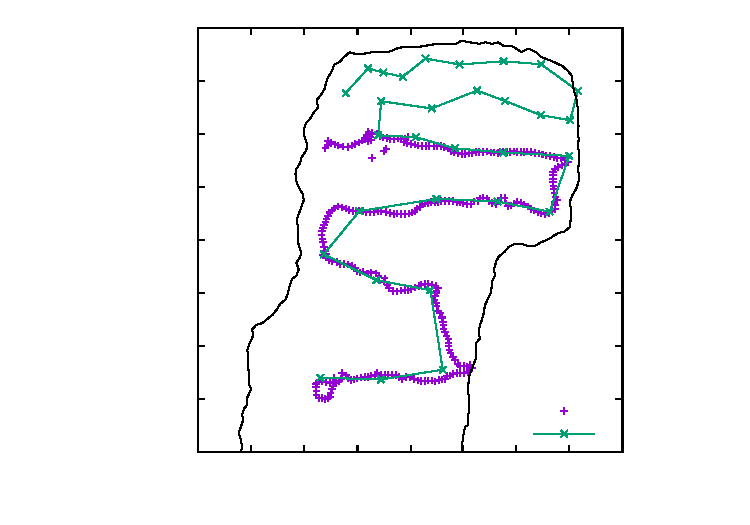
\includegraphics{GPSvsGeo}}%
    \gplfronttext
  \end{picture}%
\endgroup

\caption{Position des Bootes laut GPS-Signal verglichen mit den Messorten in Göttingen.}
\label{fig:GPSGoe}
\end{figure}



\subsection{Druck}
Da der erste Drucksensor, den wir gekauft haben, nicht wasserdicht war, nutzten wir einen, den das Institut für Geophysik in der Zwischenzeit angeschafft hat.
Er besitzt eine Schaltung, welche das Signal direkt so verstärkt, dass bei einem Druck von $1001\si{\hecto\pascal}$ eine Spannung von 1V ausgegeben wird.
Laut Datenblatt sollte der Spannungsverlauf linear mit dem Druck steigen und pro Bar ein Volt hinzubekommen.
Allerdings bemerkten wir schon während der Messung, dass die vom Datenlogger angezeigten Werte nicht ganz mit den von uns vorgenommenen Markierungen im 1m Abstand übereinzustimmen schienen.
So ließen wir die Sensoren laut Kabel bis in eine Tiefe von ca. 7.5m hinab.
Allerdings ging die tiefste Messung laut aufgezeichneten Werten unter dieser Voraussetzung nur bis in eine Tiefe von ca. 6.8m.
Da jedoch eine 8m Wassersäule schon einen beachtlichen Druck ausübt, konnten wir keine Referenzmessung zur Eichung machen, so dass wir uns entschlossen haben, einen linearen Korrekturfaktor von 1.1 einzuführen, um dem jede vermeitliche Tiefe gestreckt wird.
Unter dieser Annahme erhielten wir annehmbare Werte.
Die Linearität der Korrektur scheint in sofern angebracht, als dass wir uns bei vielen Messungen Mühe gegeben haben, die Sonde von Hand möglichst gleichmäßig herabzulassen.
Die aufgenommenen Druchkurven waren auch annähernd linear.


\subsection{Temperatur}
Die gemessene Temperatur stieg im Verlauf des Tages an der Oberfläche um ca. $xx^\circ$ an.
Dies bezieht sich auf eine Tiefe von  


\begin{figure}[h]
\centering
% GNUPLOT: LaTeX picture with Postscript
\begingroup
  \makeatletter
  \providecommand\color[2][]{%
    \GenericError{(gnuplot) \space\space\space\@spaces}{%
      Package color not loaded in conjunction with
      terminal option `colourtext'%
    }{See the gnuplot documentation for explanation.%
    }{Either use 'blacktext' in gnuplot or load the package
      color.sty in LaTeX.}%
    \renewcommand\color[2][]{}%
  }%
  \providecommand\includegraphics[2][]{%
    \GenericError{(gnuplot) \space\space\space\@spaces}{%
      Package graphicx or graphics not loaded%
    }{See the gnuplot documentation for explanation.%
    }{The gnuplot epslatex terminal needs graphicx.sty or graphics.sty.}%
    \renewcommand\includegraphics[2][]{}%
  }%
  \providecommand\rotatebox[2]{#2}%
  \@ifundefined{ifGPcolor}{%
    \newif\ifGPcolor
    \GPcolortrue
  }{}%
  \@ifundefined{ifGPblacktext}{%
    \newif\ifGPblacktext
    \GPblacktexttrue
  }{}%
  % define a \g@addto@macro without @ in the name:
  \let\gplgaddtomacro\g@addto@macro
  % define empty templates for all commands taking text:
  \gdef\gplbacktext{}%
  \gdef\gplfronttext{}%
  \makeatother
  \ifGPblacktext
    % no textcolor at all
    \def\colorrgb#1{}%
    \def\colorgray#1{}%
  \else
    % gray or color?
    \ifGPcolor
      \def\colorrgb#1{\color[rgb]{#1}}%
      \def\colorgray#1{\color[gray]{#1}}%
      \expandafter\def\csname LTw\endcsname{\color{white}}%
      \expandafter\def\csname LTb\endcsname{\color{black}}%
      \expandafter\def\csname LTa\endcsname{\color{black}}%
      \expandafter\def\csname LT0\endcsname{\color[rgb]{1,0,0}}%
      \expandafter\def\csname LT1\endcsname{\color[rgb]{0,1,0}}%
      \expandafter\def\csname LT2\endcsname{\color[rgb]{0,0,1}}%
      \expandafter\def\csname LT3\endcsname{\color[rgb]{1,0,1}}%
      \expandafter\def\csname LT4\endcsname{\color[rgb]{0,1,1}}%
      \expandafter\def\csname LT5\endcsname{\color[rgb]{1,1,0}}%
      \expandafter\def\csname LT6\endcsname{\color[rgb]{0,0,0}}%
      \expandafter\def\csname LT7\endcsname{\color[rgb]{1,0.3,0}}%
      \expandafter\def\csname LT8\endcsname{\color[rgb]{0.5,0.5,0.5}}%
    \else
      % gray
      \def\colorrgb#1{\color{black}}%
      \def\colorgray#1{\color[gray]{#1}}%
      \expandafter\def\csname LTw\endcsname{\color{white}}%
      \expandafter\def\csname LTb\endcsname{\color{black}}%
      \expandafter\def\csname LTa\endcsname{\color{black}}%
      \expandafter\def\csname LT0\endcsname{\color{black}}%
      \expandafter\def\csname LT1\endcsname{\color{black}}%
      \expandafter\def\csname LT2\endcsname{\color{black}}%
      \expandafter\def\csname LT3\endcsname{\color{black}}%
      \expandafter\def\csname LT4\endcsname{\color{black}}%
      \expandafter\def\csname LT5\endcsname{\color{black}}%
      \expandafter\def\csname LT6\endcsname{\color{black}}%
      \expandafter\def\csname LT7\endcsname{\color{black}}%
      \expandafter\def\csname LT8\endcsname{\color{black}}%
    \fi
  \fi
  \setlength{\unitlength}{0.0500bp}%
  \begin{picture}(7200.00,5040.00)%
    \gplgaddtomacro\gplbacktext{%
      \csname LTb\endcsname%
      \put(814,704){\makebox(0,0)[r]{\strut{} 15}}%
      \put(814,1518){\makebox(0,0)[r]{\strut{} 20}}%
      \put(814,2332){\makebox(0,0)[r]{\strut{} 25}}%
      \put(814,3147){\makebox(0,0)[r]{\strut{} 30}}%
      \put(814,3961){\makebox(0,0)[r]{\strut{} 35}}%
      \put(814,4775){\makebox(0,0)[r]{\strut{} 40}}%
      \put(1380,484){\makebox(0,0){\strut{} 0}}%
      \put(2464,484){\makebox(0,0){\strut{} 0.5}}%
      \put(3549,484){\makebox(0,0){\strut{} 1}}%
      \put(4634,484){\makebox(0,0){\strut{} 1.5}}%
      \put(5718,484){\makebox(0,0){\strut{} 2}}%
      \put(6803,484){\makebox(0,0){\strut{} 2.5}}%
      \put(176,2739){\rotatebox{-270}{\makebox(0,0){\strut{}$T\, [\si{\celsius}]$}}}%
      \put(3874,154){\makebox(0,0){\strut{}$z$ [m]}}%
    }%
    \gplgaddtomacro\gplfronttext{%
      \csname LTb\endcsname%
      \put(5816,1097){\makebox(0,0)[r]{\strut{}Messwerte (ohne Ausreißer)}}%
      \csname LTb\endcsname%
      \put(5816,877){\makebox(0,0)[r]{\strut{}Approximation}}%
    }%
    \gplbacktext
    \put(0,0){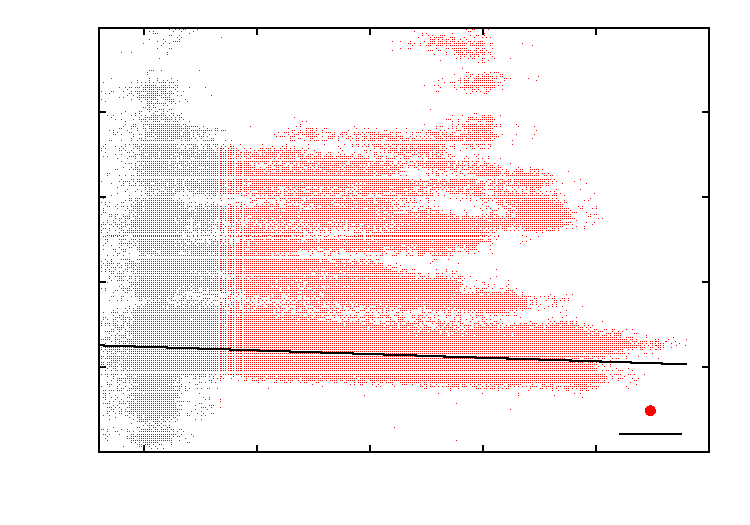
\includegraphics{temp_goe}}%
    \gplfronttext
  \end{picture}%
\endgroup

\caption{Temperaturverlauf am Göttinger Kiessee mit fast allen aufgenommenen Werten. Einige Werte, welche offensichtlich durch Wackelkontakte zu stande kommen (bis zu $140^\circ$C) wurden zwecks Übersichtlichkeit ausgeblendet.}
\label{fig:temp_goe}
\end{figure}


\subsection{Gemessenes Abstandsgesetz}
Da nun die Sendeleistung nicht ausreichte, um die Anordnung der Piezokristalle tatsächlich als Echolot zu verwenden haben wir die Abstandsabhängigkeit der Schallintensität näher untersucht. 
Dies wurde zunächst mit der Motivation durchgeführt eine mit der vorgegebenen Sendeleistung maximale Reichweite zu ermitteln. Als klar wurde, dass diese nicht ausreichen wird haben wir
die Abnahme der Amplitude weiter untersucht.

Zu diesem Zweck haben wir die Sender parallel zueinander ausgerichet und den Abstand mit einer Skala gemessen. Um dann die Amplitude bei einer bestimmten Entfernung abzulesen, haben wir ein
ein Oszilloskop verwendet.

Wir haben hierfür drei Messreihen durchgeführt, dann wurde für jede Entfernung der Mittelwert mit Standardabweichung berechnet. In Grafik \ref{fig:schall} ist das Messergebnis zu sehen, wobei wir die relative Amplitude $\frac{I}{I_0}$ berechnet haben.

\begin{figure}[h]
	\centering
	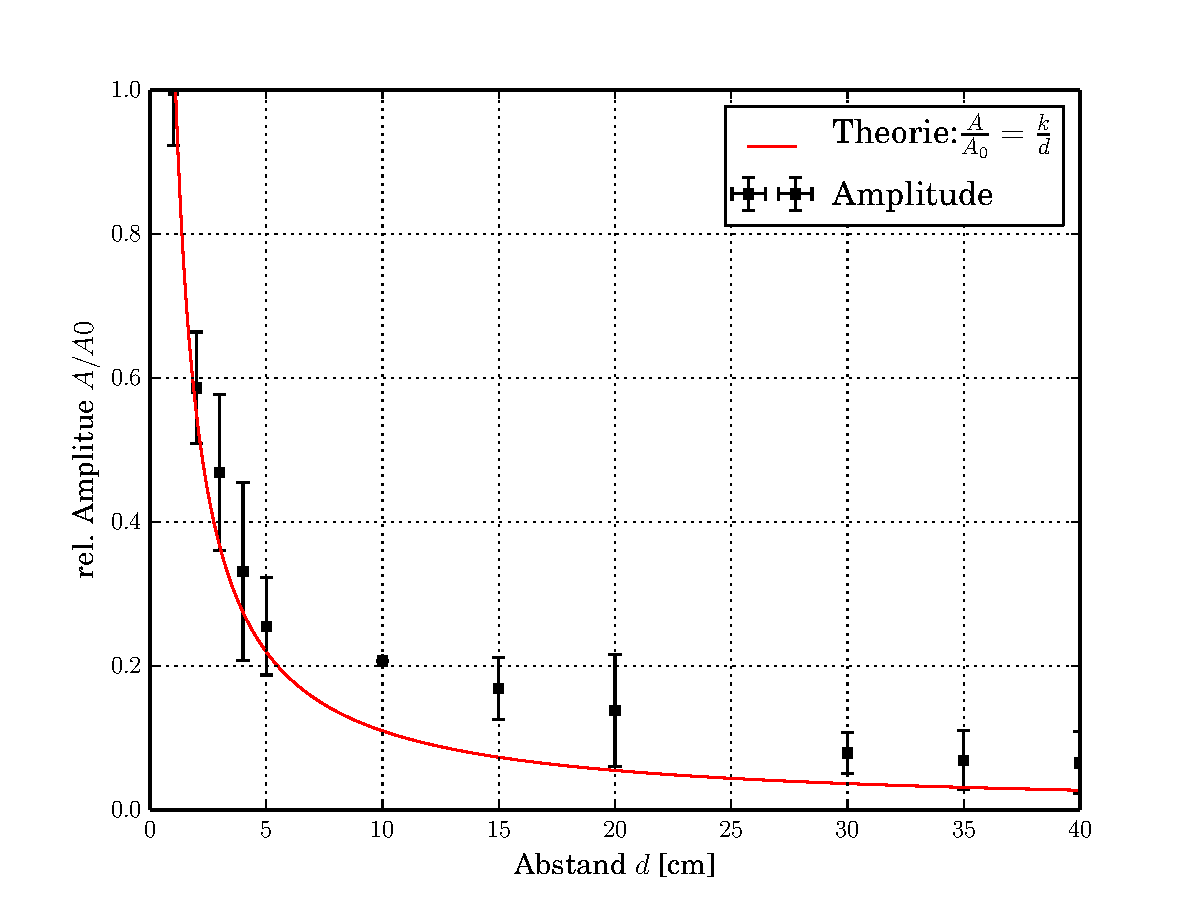
\includegraphics[width=0.8\textwidth]{schall.pdf}
	\caption{Relative Amplitude wurde aufgetragen gegen den Abstand $d$. Zudem wurde eine $\chi^2$ Anpassung an die Messdaten durchgeführt.}
	\label{fig:schall}
\end{figure}

Zudem wurde eine $\chi^2$ Anpassung an die berechneten Mittelwerte durchgeführt, wobei hier die in der Theorie vorgestelle $\frac{1}{d}$ - Abhängigkeit angenommen wurde.
Es wurde hier also angenommen, dass die mit dem Oszilloskop gemessene Amplitude sich wie die Abstandsabhängigkeit des Schalldrucks verhält.
Dies erscheint sinnvoll, denn entscheidend für die angezeigte Amplitude ist, welche Beschleunigungen auf den Empfänger wirken.


Da die eingezeichneten Fehlerbalken sich nur aus der statistischen Standardabweichung berechnen muss davon ausgegen werden, dass die Messung eigentlich noch ungenauer waren. Diese Abhängigkeit war auch hier recht gut gegeben, wie man in dem Plot erkennen kann. 
Man kann gut erkennen, dass die Amplitude nach gerade einmal circa 2,5 cm auf unter die Hälfte abgefallen ist. Bei einer Entfernung von 40 cm ist dann nur noch gut 5 $\%$ vorhanden. Es wird also sehr deutlich, dass die Sendeleistung nicht ausreichen würde für die geplanten Versuche, denn innerhalb eines homogenen Mediums liegt stets eine $\frac{1}{d}$ -Abhängigkeit vor (vgl. Theorie). 


\section{Diskussion}
\label{sec:diskussion}

\subsection{Refferenzspsnnung des ADC}
Für den ADC wurde die Interne Refferenzspannung des Controllers verwendet.
Diese ist aber durch den normalen Betrieb des Controllers ein klein wenig verrauscht und verrauscht somit auch die ADC Werte.
Dies hat eine Größenordnung von etwa 5\si{\milli\volt} und ist in allen Datensätzen zu sehen.
Um diesen Fehler zu beheben bzw. zu verringern ist es nötig eine konstante Refferenzspannung zu verwenden.
Das Board hat einen nach außen geführten Pin für die Refferenzspannung.
Nun ist es nötig entweder die 3.3\si{\volt} des Boards zu nehmen, oder eine eigene Spannungsquelle zu bauen.
An egal welcher der beiden Quellen darf dann auch keine weitere Last liegen, um die Spannung so konstant wie möglich zu halten.
Zu den muss ein Tiefpassfilter mithilfe einer Drosselspule in Reihe geschaltet werden um das durch die Elektronik induzierte Rauschen zu unterdrücken.

\subsection{Druck}


\subsection{Echolot}
Die Idee des Echolots konnte nicht vollständig umgesetzt werden, da das Signal nicht stark genug war, um bis in eine Tiefe von etwa 6\si{\meter} einzudringen und reflektiert zu werden.
Um in diese Vordringen zu können müsste mehr Schalldruck erzeugt werden und dazu ist eine größere physische Ausdehnung des Kristalles nötig.
Dies kann entweder durch das Verwenden von einer höheren Spannung am Sender oder durch das Verwenden einer H-Brücke getan werden.
Letzteres sorgt für das Verwenden von $\pm24\si{\volt}$, welches zur doppelten physischen Ausdehnung des Kristalls sorgt.
Dies kann weiterhin verstärkt werden, in dem bis zu 48\si{\volt} angelegt werden.
Der Nachteil der H-Brücke ist, dass bei jedem Umschalten die Schlatung kurzgeschlossen wird, was unterbunden werden muss, da die MosFet Transistoren mit einer Frequenz von 40\si{\kilo\hertz} versorgt werden.
Wir haben dennoch ein paar Testdaten aufnehmen und Auswerten können.

\subsection{Ortsbestimmung}
Bei der ersten Messung haben wir den Ort mit einem Geodimeter bestimmt.
Problematisch war hierbei, dass das Boot mit dem Spiegel relativ stark geschwankt hat.
Dies führte gerade bei Messungen, wo das Boot relativ dicht am Geodimeter war dazu, dass die Aufnahme der Position schwer war.
An einer Stelle konnten wir den Messstab in über 5 min nicht ruhig genug halten, so dass wir schließlich die Position nicht aufnahmen.
Generell war es ein Problem, dass wir nur zwei Leute auf dem Boot hatten: einen Ruderer, der während der Messung den Stab hochgehalten hat und einen, der sich um die Sonde kümmerte.
Dies führte dazu, dass häufig der für den Retroreflektor zuständige diesen zu schräg hielt, so dass die Spiegelfläche nicht sichtbar war.
Da wir bei der Messung die Funkgeräte vergessen hatten, mussten wir uns mit Handzeichen verständigen.
Dies stellte selbst am Göttinger Kiessee an den entferntesten Messpunkten eine Herausforderung dar, so dass dort das Boot-Team häufig unnötig lange an einem Ort blieb, da sie die Bestätigung nicht sahen.


Außerdem behindert am Seeburger See eine Insel ein großteil des Blickfelds.

Es stellte sich bei den Messungen heraus, dass die Genauigkeit des Geodimeters keine Rolle spielte, da das Boot von Wind und Strömung während der Messung sehr stark abgetrieben wurde.
Daher setzten wir bei der zweiten Messung unsere erste Idee um, die Position über GPS zu erfassen funktioniert, welche wir wegen der vermeitlich schlechten Auflösung von 5-10m verwarfen.

\subsection{Temperatur}
Bei der zweiten Messung zeigte sich in den Daten, dass die Werte der Temperatur augenscheinlich gleichzeitig drei Werte annehmen.
Bei genauerer Betrachtung der Messwerte fällt jedoch auf, wie in Abb. \ref{fig:tempSprung} zu erkennen, dass jeweils ungefähr 10 Messwerte auf einem niedrigen, dann auf einem mittleren, erneut auf einem niedrigen und dann wieder auf einem hohen Niveau liegen.
Dies  entspricht genau der Frequenz, mit der wir die LEDs angeschaltet haben (keine LED, blaue LED, keine LED, IR-LED).
Für beide Messungen benutzten wir den Micro-Controller als Stromquelle.
Dieser ist für Ströme von bis zu 350mA ausgelegt.
Augenscheinlich haben da die 50mA, welche die LEDs benötigten, die Stromzufuhr des PT1000 so stark beeinflusst, dass die aufgenommenen Messwerte Temperatursprünge von biszu $4^\circ $C aufweisen.

\begin{figure}[h]
	\centering
	% GNUPLOT: LaTeX picture with Postscript
\begingroup
  \makeatletter
  \providecommand\color[2][]{%
    \GenericError{(gnuplot) \space\space\space\@spaces}{%
      Package color not loaded in conjunction with
      terminal option `colourtext'%
    }{See the gnuplot documentation for explanation.%
    }{Either use 'blacktext' in gnuplot or load the package
      color.sty in LaTeX.}%
    \renewcommand\color[2][]{}%
  }%
  \providecommand\includegraphics[2][]{%
    \GenericError{(gnuplot) \space\space\space\@spaces}{%
      Package graphicx or graphics not loaded%
    }{See the gnuplot documentation for explanation.%
    }{The gnuplot epslatex terminal needs graphicx.sty or graphics.sty.}%
    \renewcommand\includegraphics[2][]{}%
  }%
  \providecommand\rotatebox[2]{#2}%
  \@ifundefined{ifGPcolor}{%
    \newif\ifGPcolor
    \GPcolorfalse
  }{}%
  \@ifundefined{ifGPblacktext}{%
    \newif\ifGPblacktext
    \GPblacktexttrue
  }{}%
  % define a \g@addto@macro without @ in the name:
  \let\gplgaddtomacro\g@addto@macro
  % define empty templates for all commands taking text:
  \gdef\gplbacktext{}%
  \gdef\gplfronttext{}%
  \makeatother
  \ifGPblacktext
    % no textcolor at all
    \def\colorrgb#1{}%
    \def\colorgray#1{}%
  \else
    % gray or color?
    \ifGPcolor
      \def\colorrgb#1{\color[rgb]{#1}}%
      \def\colorgray#1{\color[gray]{#1}}%
      \expandafter\def\csname LTw\endcsname{\color{white}}%
      \expandafter\def\csname LTb\endcsname{\color{black}}%
      \expandafter\def\csname LTa\endcsname{\color{black}}%
      \expandafter\def\csname LT0\endcsname{\color[rgb]{1,0,0}}%
      \expandafter\def\csname LT1\endcsname{\color[rgb]{0,1,0}}%
      \expandafter\def\csname LT2\endcsname{\color[rgb]{0,0,1}}%
      \expandafter\def\csname LT3\endcsname{\color[rgb]{1,0,1}}%
      \expandafter\def\csname LT4\endcsname{\color[rgb]{0,1,1}}%
      \expandafter\def\csname LT5\endcsname{\color[rgb]{1,1,0}}%
      \expandafter\def\csname LT6\endcsname{\color[rgb]{0,0,0}}%
      \expandafter\def\csname LT7\endcsname{\color[rgb]{1,0.3,0}}%
      \expandafter\def\csname LT8\endcsname{\color[rgb]{0.5,0.5,0.5}}%
    \else
      % gray
      \def\colorrgb#1{\color{black}}%
      \def\colorgray#1{\color[gray]{#1}}%
      \expandafter\def\csname LTw\endcsname{\color{white}}%
      \expandafter\def\csname LTb\endcsname{\color{black}}%
      \expandafter\def\csname LTa\endcsname{\color{black}}%
      \expandafter\def\csname LT0\endcsname{\color{black}}%
      \expandafter\def\csname LT1\endcsname{\color{black}}%
      \expandafter\def\csname LT2\endcsname{\color{black}}%
      \expandafter\def\csname LT3\endcsname{\color{black}}%
      \expandafter\def\csname LT4\endcsname{\color{black}}%
      \expandafter\def\csname LT5\endcsname{\color{black}}%
      \expandafter\def\csname LT6\endcsname{\color{black}}%
      \expandafter\def\csname LT7\endcsname{\color{black}}%
      \expandafter\def\csname LT8\endcsname{\color{black}}%
    \fi
  \fi
    \setlength{\unitlength}{0.0500bp}%
    \ifx\gptboxheight\undefined%
      \newlength{\gptboxheight}%
      \newlength{\gptboxwidth}%
      \newsavebox{\gptboxtext}%
    \fi%
    \setlength{\fboxrule}{0.5pt}%
    \setlength{\fboxsep}{1pt}%
\begin{picture}(7200.00,5040.00)%
    \gplgaddtomacro\gplbacktext{%
      \csname LTb\endcsname%
      \put(682,1126){\makebox(0,0)[r]{\strut{}$18$}}%
      \put(682,1886){\makebox(0,0)[r]{\strut{}$19$}}%
      \put(682,2647){\makebox(0,0)[r]{\strut{}$20$}}%
      \put(682,3407){\makebox(0,0)[r]{\strut{}$21$}}%
      \put(682,4168){\makebox(0,0)[r]{\strut{}$22$}}%
      \put(1738,484){\makebox(0,0){\strut{}$3300$}}%
      \put(2925,484){\makebox(0,0){\strut{}$3320$}}%
      \put(4112,484){\makebox(0,0){\strut{}$3340$}}%
      \put(5300,484){\makebox(0,0){\strut{}$3360$}}%
      \put(6487,484){\makebox(0,0){\strut{}$3380$}}%
    }%
    \gplgaddtomacro\gplfronttext{%
      \csname LTb\endcsname%
      \put(176,2739){\rotatebox{-270}{\makebox(0,0){\strut{}$^\circ$ C}}}%
      \put(3808,154){\makebox(0,0){\strut{}Messpunkt}}%
      \csname LTb\endcsname%
      \put(5816,4602){\makebox(0,0)[r]{\strut{}Temperatur}}%
    }%
    \gplbacktext
    \put(0,0){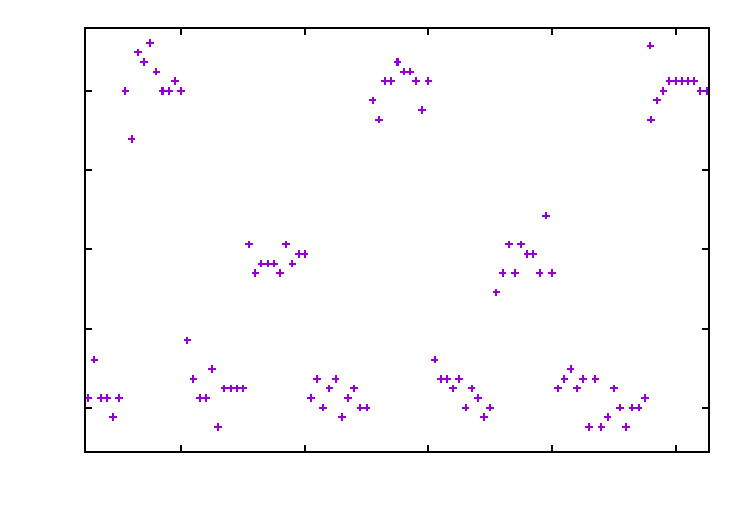
\includegraphics{tempSprung}}%
    \gplfronttext
  \end{picture}%
\endgroup

	\caption{Vergrößerte Darstellung einer Temperaturkurve.}
	\label{fig:tempSprung}
\end{figure}



\subsection{Absorption}
Bei der Messung der Absorbtion stellte sich sehr schnell heraus, dass die Daten stark verrauscht sind, besonders an der Oberfläche des Wassers.
Dies liegt wahrscheinlich daran, dass durch die Bewegung der Wasseroberfläche das Sonnenlicht besser und schlechter Reflektiert wird.
Um dieses hochfrequente Rauschen zu unterdrücken kann der Strom der Photodiode zusätzlich noch durch einen Tiefpassfilter geleitet werden.
Hierzu müsste nur eine Drosselspule in Reihe mit der Photodiode und dem ADC geschaltet werden.
Somit werden nur die niederfrequenten Änderungen des Photostroms aufgezeichnet.


\subsection{Messprobleme und verworfene Ideen}
Unsere erste Idee war die, ein ferngesteuertes U-Boot zu bauen, was die Sensoren an Bord hat.
Dies stellte sich jedoch sehr schnell als nicht durchführbar heraus, da es keine geeigneten Modellbauten gab und da die komplette Technik mit Stromversorgung unter Wasser luftdicht sein müsste.
Daher kamen wir auf die Idee, eine ferngesteuerte Plattform zu bauen, welche die Sonden mit einer Winde ferngesteuert herunterlässt.
Dies verwarfen wir jedoch auch sehr schnell, da die Fernsteuertechnik einen großen Teil unserer Arbeit ausgemacht hätte, was wissenschaftlich wenig interessant ist.
Auch hätten wir Probleme bekommen, falls sich zum Beispiel die Sensoren in Wasserpflanzen verfangen.

So entschieden wir uns für die simplere Umsetzung, ein Ruderboot zu nehmen und die Stromversorgung, sowie die Datenverarbeitung im Boot zu betreiben und nur die Sensoren an den Kabeln herunter zu lassen.


Wir hatten zunächst noch vor, weitere Sensoren zu verwenden:
\begin{itemize}
	\item \textit{el. Leitfähigkeit}: Funktionierte nicht, da wir dafür Wechselspannungen mit mindestens 50V benötigt hätten.
		Dies wäre notwendig, da sich sonst an den Elektroden durch Eletrolyse Salze angelagert hätten, welche für eine höhere gemessene Leitfähigkeit gesorgt hätten.
		Die Leitfähigkeit alleine ist kein Maß für den Salzgehalt, der auch noch von anderen Größen maßgeblich beeinflusst wird.
		So konnten wir den Sensor, welchen Jan bereits besorgt hatte, nicht einsetzen.
	\item \textit{pH-Wert}: Der pH-Wert wäre auch eine interessante Messgröße gewesen.
		Allerdings wäre zur Kallibration mindestens eine Pufferlösung notwendig gewesen.
		Ausschlaggebend war, dass wir zu den preislich akzeptablen Sensoren keine vernünftigen Datenkurven finden konnten, da diese augenscheinlich nur für fertige Geräte ausgelegt sind.
\end{itemize}


\bibliography{literatur}
\bibliographystyle{babalpha}
\end{document}
